\documentclass[12pt]{article}
\usepackage[a4paper, total={6in, 9in}]{geometry}
\usepackage{titling}
\usepackage{amsmath,amsfonts,amssymb}
\usepackage{enumerate}% http://ctan.org/pkg/enumerate
\usepackage{apacite}
\usepackage{braket}
\usepackage{booktabs}
\usepackage[table,xcdraw]{xcolor}
\usepackage[toc,page]{appendix}
\newcounter{para}[subsection]
\usepackage[round]{natbib}
\newcommand{\aap}{A\&A}
\newcommand{\icarus}{icarus}
\newcommand{\mnras}{Monthly Notices of the RAS}
\usepackage{graphicx}
\usepackage{subcaption}
\usepackage{floatrow}
\usepackage[export]{adjustbox}[2011/08/13]
\usepackage{fancyhdr}
\pagestyle{fancy}
%\lhead{Nam HOANG}
\rhead{}
%\renewcommand{\headrulewidth}{0.4pt}
%\renewcommand{\footrulewidth}{0.4pt}
\usepackage[colorlinks]{hyperref}
\AtBeginDocument{%
	\hypersetup{
		citecolor=blue,
		linkcolor=blue,   
		urlcolor=magneta}}


\title{Geological Constraints on Astronomical Solutions}
\author{Nam HOANG}
\begin{document}
	%    \begin{titlingpage}
	%        \maketitle 
	%        \begin{abstract}
	%            For over a century, fingerprints have been an undisputed
	%            personal identifier.  Recent court rulings have sparked
	%            interest in verifying unique techniques to make the current
	%            methods even more reliable. Ducks, as they do not have
	%            fingers, play a key role in the development of new methods to
	%            protect the innocent of our society.
	%        \end{abstract}
	%    \end{titlingpage}    
	%%    
	\begin{titlepage}
		\begin{figure}[t]
			\centering\includegraphics[width=0.4\textwidth]{logo-obspm-imcce.png}  \hfill
			\centering\includegraphics[width=0.4\textwidth]{logo_ens_2010.jpg}
		\end{figure}
		%        \centering\includegraphics[width=0.3\textwidth]{logo-obspm-imcce.png}
		
		%    \begin{center}
		%        \includegraphics[width = 20mm]{"logo-obspm-imcce.png"} \hfill
		%        \includegraphics[width = 20mm]{"logo_ens_2010.jpg"}
		%    \end{center}
		%        \includegraphics[width = 20mm]{Im3.jpg}
		
		\begin{center}
			\textsc{ \LARGE{Ecole Normale Superieure de Lyon \\}}
			\textsc{ \LARGE{Master 2 Science de la Matiere\\ }}
			\textnormal{ \LARGE{Physique, concepts et applications\\}}
			\vspace{30mm}
			\fontsize{10mm}{7mm}\selectfont 
			\textup{Geological Constraints \\on Past Dynamics of Solar System Planets}\\
		\end{center}
		\vspace{75mm}
		
		
		\begin{minipage}[t]{0.47\textwidth}
			\textnormal{\large{\bf Supervisors:\\}}
			{\large Prof. Jacques Laskar\\ Dr. Federico Mogavero}
		\end{minipage}\hfill\begin{minipage}[t]{0.47\textwidth}\raggedleft
			\textnormal{\large{\bf Student:\\}}
			{\large Nam HOANG }
		\end{minipage}
		
		\vspace{25mm}
		
		\centering{\large{Academic year 2018/2019 \\ Paris - \today }}
		
	\end{titlepage}
	
	\begin{abstract}
		Variations in the Earth's orbit govern the insolation and its climate. The astronomical signals, which have been recovered in geological records \citep{hays1976}, revolutionized the accuracy and precision of determination of the geological time scale \citep{gradstein2012}. The orbital variations beyond 50 Myr cannot be reliably predicted because of the chaotic dynamics of the Solar System \citep{laskar1989}. However, the chaotic orbital evolution in the past could be constrained by geological data: Among 11 possible different astronomical evolutions, one was found to match the Newark-Hartford (NH) data from 210 Myrs ago \citep{olsen2019}, another one matches the resonance transition observed in Libsack dated back to 87 Myrs ago \citep{ma2017}. With 10,000 numerical integrations of 300 Myr from averaged equations of simplified Solar System, we have found several solutions that match better with the NH data, and a robust mechanism of the transition in Libsack record. Statistical analysis was also performed to obtain the probability density functions (PDF) of fundamental frequencies of the Solar System, that could be roughly approximated by Gaussian functions. The evolution of the PDF is found to be similar to the one of a diffusive process.
		
	\end{abstract}
	\newpage
	\section*{Acknowledgements}
	I would like to express my gratitude to my supervisor Jacques Laskar for his fruitful discussion and productive guide, to my friend Federico Mogavero for the enjoyable companionship and the great support on this work. I thank ENS de Lyon for providing me the scholarship and their exceptional master program. 
	
	\newpage
	\tableofcontents
	\newpage
	\listoffigures
	\listoftables
	\newpage
	\section{Introduction} 
	\subsection{Orbital dynamics}
	The Solar System planets conform to Kepler's law in the first order of approximation. Sizes and shapes of the orbits are described by semi-major axis $a$ and eccentricity $e$; their orientations in space are determined by the inclination $I$, the longitude of ascending node $\Omega$ and the argument of perihelion $\omega$; while the position of the planet on orbit is described by the mean anomaly $M$. These variables are called orbital elements, which are all constant in Kepler's orbits except for $M$, which increases linearly with time with mean motion $n = dM/dt$. However, these ``constant" orbital elements actually change with time, although the rate is much smaller than mean motion $n$. More precisely, all the orbital components can be approximated as a series of secular fundamental frequencies, representing roughly the contribution of each planet to orbital deformation. These frequencies portray the precession of perihelion ($g_j$ frequencies) and precession of the orbital plane in space ($s_j$ frequencies), where $j$ numbers the planet in ascending order of radial distance from the Sun.
	
	
	The long term variation of planetary orbital elements is induced by many factors: relativistic corrections, non-spherical Sun, tidal effects, etc. But the main cause is the planet-planet gravitational interactions. Therefore, a simple Newtonian model of Solar System consisting of 8 planets could already give a good approximation of $g_i$ and $s_i$.
	The first calculation of secular orbital variation was done by \cite{lagrange1782theorie}. The secular approach rests on two main ideas: the Hamiltonian is first expanded in small parameters, which are mass, eccentricity and inclination; rapidly-changing variables are then averaged (mean anomaly $M$ in this case) to obtain a so-called secular Hamiltonian. Since Lagrange, a secular model of the Solar System has been greatly improved (notably by \cite{le1856} and \cite{Hill1873}).
	Recently, analytic theory of the regular secular motion of 8 planets was given by \cite{bretagnon1974termes}, where the Hamiltonian was expanded up to order 2 in planetary mass and degree 4 in eccentricity and inclination. In his perturbative approach, he assumed the dynamics to be regular, and to have quasi-periodic solutions.
	\citet{laskar1985} had a different approach. He first computed the secular Hamiltonian up to order 2 in planetary mass and degree 6 in eccentricity and inclination. The secular equations PDF then numerically integrated up to 200 Myr, which could be done effectively by taking a large time step of 500 years because of the averaging nature of this secular approach. By virtue of this long integration, \cite{laskar1989} was able to calculate the largest Lyapunov exponent of the Solar System to be around 1/5 $\text{Myr}^{-1}$, indicating that the orbital evolution is chaotic. This was later confirmed by \cite{sussman1992}, who also showed that the integration of giant planets, namely Jupiter, Saturn, Uranus, and Neptune, are by themselves chaotic, although in a much lesser way.
	
	Long term direct integration of a realistic model of the Solar System is first realized by \cite{quinn1991} over 3 Myr, which confirmed perfectly the secular solution. Until now, the Solar System could be integrated over its expected time-life (5 Gyr) \citep{Laskar2009}. Nevertheless, the solutions remain predictive only during 60 Myr from the present. The origin of this limit is less a matter of initial conditions precision than the chaotic nature of the Solar System. The uncertainty, which is very small initially, always diverges exponentially; it actually grows 10-fold every 10 Myr. This exponential divergence discourages any hope of having a deterministic picture of Solar System into the far past or into the far future. However, a reliable statistical picture of the Solar System is feasible over a long timescale. \cite{laskar2008} performed a statistical analysis over 1001 different integration of secular equation over 5 Gyr. The probability density function (PDF) of gaseous planets PDF found to be close to that of quasi-periodic motion. More interestingly, the PDF evolution of terrestrial planets are perfectly fitted by a Rice distribution; they are similar to the one of a diffusive process that could be simply modeled by a random walk approach. Using a different approach, \cite{federico2017} considered the planet orbits as a statistical ensemble with the conservation of total energy and total angular momentum. He produced the stationary PDF of the inner planets, which remarkably resembled the numerical PDF of \cite{laskar2008} except for Mercury; this result demonstrates that the orbital elements of the planets are indeed randomized by the chaos.
	
	\subsection{Milankovitch cycles}
	
	\citet{milankovitch1941canon} hypothesized that the origin of large climate change on Earth originates from the long-term variation of its orbital elements through insolation. The astronomical evolution directly modulates the insolation on Earth. For example, combinations of the $g_i$  and the axial precession $p$  represent the so-called "climatic precession" frequency of insolation, averaging about 20 kyr at the present.
	Difference between $g_i$ generate the frequencies of eccentricity; these are known as eccentricity cycles, which comprise short cycles of 100 kyr, 405-kyr long cycle and grand cycles, longest of which is $g_4-g_3$, numbering around 2.4 Myr.
	Likewise, the difference between $s_i$ and p yield the obliquity periods. These cycles are collectively called Milankovitch cycles.
	
	The first evidence of this theory was reported by \cite{hays1976}, where they found a correlation between astronomical forcing and the $\delta^{18} \text{O}$ (a measure of ratio of $ {}^{18} \text{O} $ and $ {}^{16} \text{O} $  ) records over the past 500 kyr. 
	Since then, interest in the theory surged as many geological records of climate responding to insolation forcing have been found, which confirmed the Milankovitch theory of paleoclimate (see \citealt{imbrie1982} for more historical details). This correlation between precise astronomical solutions and often noisy geological data also provide an excellent way of dating the data, which becomes standard practice in the stratigraphic community. The most recent standard geological timescale (\cite{gradstein2004},\cite{gradstein2012}) incorporates the astronomical calibration of the Neogen period through La2004 solution \citep{laskar2004}. 
	\subsection{Resonance and Chaos in Solar System}
	An integrable system could always be described by a set of action-angle variables, where action variables stay constant and angle variables increase linearly with time with a constant rate $\theta_i$, which are known as fundamental frequencies of the system. 
	A resonance occurs when a linear combination of two or more fundamental frequencies of the system: $\sigma = \sum p_i \theta _i $ (where $\theta$ are frequencies and $p_i$'s are integers) is nearly zero. A system is said to be in resonance if the angle corresponding to $\sigma$ experiences a bounded oscillation around the center of resonance, where $\sigma$ is exactly zero; in which case, the angle librates. When said angle increases or decreases indefinitely, the system is not in resonance with $\sigma$, the motion is called circulation. The trajectory dividing libration and circulation in phase space is called separatrix. Chaos in a Hamiltonian system occurs when a separatrix of resonance is disturbed by another resonance. Therefore, to understand chaos, it is crucial to understand the network of resonance and their possible overlap.  
	
	%    Since the work of Sussman proving that the giant planets are by themselves chaotic, Murray and Holman (?) have found an overlapping cluster of mean motion resonances between Jupiter, Saturn and Uranus, that could explain the chaotic motion of the Outer Solar System. 
	Laskar et al. (1990, 1992) presented several secular resonances as a candidate source of chaos for Inner Solar System, :
	\begin{align}
	\theta_1 &= 2(g_4 - g_3) - (s_4 - s_3), \\ 
	\theta_2 &= (g_4 - g_3) - (s_4 - s_3), \\
	\sigma &= (g_1 - g_5) - (s_1 - s_2).
	\end{align}
	He observed that (1) the angles corresponding to $\theta_1$ and $\sigma$ are presently librating, but will progress to a circulation state around -50 Myr, (2) it's highly probable that $\theta_1$ will transition to another resonance $\theta_2$.
	Although these secular resonances can interact with each other and form chaotic overlaps (especially between $\theta_1$ and $\theta_2$), a direct and robust mechanism causing large scale chaos is still missing. Therefore the origin of chaos in the Inner Solar System remains an open question.
	
	
	\subsection{Review of Literature }
	
	The chaotic nature of Solar System implies that astronomical calibration of the geological record is only credible in the Cenozoic era (66 Myr ago to now), and must be done with caution for the Mesozoic era (252 Myr to 66 Myr ago) or later. Only with numerical integration from present initial conditions, the picture of Solar System becomes fuzzy after 60 Myr with countless possibilities. \cite{olsen2019} show that this picture of Solar System could be made cleaner by geological records. They first presented long continuous lacustrine data dating from 199 Myr to 220 Myr ago, which was collected by the Newark Basin Coring Project. The Newark-Hartford (NH) data was then dated by the relatively stable 405-kyr McLaughlin cycle ($g_2 - g_5$), and complimentarily verified by other timing methods. Except for the part whose period longer than 405 ky, the spectrum of the geological data and the spectrum of the present eccentricity of the Earth shows overall agreement including the 20-kyr precessional and the 100-kyr short eccentricity cycles; this agreement was later confirmed by a more precise frequency analysis \citep{laskar1993FA}. They later asserted that the discrepancies PDF the result of chaotic diffusion, i.e the drift of fundamental frequencies over time. A particular solution La2010d \citep{laskar2010} was found to offset the frequency discrepancies and showed incredible agreement with the geological record. A further statistical test was done to demonstrate that Newark-Hartford data resulting from chaotic diffusion is a very likely probability.
	
	Geological evidence of chaotic dynamical behavior of Solar System was also reported from Libsack core of Cretaceous basin, which dates back to 83-90 Myr ago \citep{ma2017}. From the spectrum analysis of the data, a sudden change of a long cycle period from 2.4 Myr to 1.2 Myr was observed. The initial 2.4 Myr cycles PDF attributed to the grand eccentricity cycle 2 $(g_4-g_3)$, and 1.2 Myr to $(g_4-g_3)$. With the recorded inclination cycle $(s_4-s_3)$ remained unchanged, the transition from the $\theta_1$ resonance to the $\theta_2$ resonance was therefore apparent from the geological data. Interestingly, the La2004 solution \citep{laskar2004}, not La2010d, exhibits the resonance transition from $\theta_1$ to $\theta_2 $  during approximately the same time as Libsack core. It's thus highly possible that there exists an ensemble of solutions, which will be able to explain both the irregular characteristics of Libsack data and Newark-Hartford data.
	
	\subsection{End goal and plan}
	The end goal of this project is in line with the objectives of the two papers presented above. By using the geological records as constraints, we want to break through the 60-Myr barrier of predictability to anchor the fundamental frequencies beyond this range. We aim to have a template for an astronomical orbital solution that could be used in the astronomical calibration of additional geological data over the Mesozoic Era. In order to achieve this, we need precise frequency constraints which require a long, continuous and well-defined data, the core from Newark-Hartford basins is among the few that are exceptional in this regard. As good as it is, the uncertainty of frequencies obtained from the cores is still difficult to obtain, therefore the exact ``error bars" are still missing. Another obstacle is the enormous computational power required to directly integrate the complete astronomical equations; it takes 4 months to get a single solution over 250 Myr by a 6-core processor. This obstacle should be tackled directly in the future study to obtain the solutions that fit the available geological data.
	
	This preliminary study made use of the secular equations for faster integrations, which is also the initial phase of the larger project to achieve the end goal. \cite{olsen2019} have found    11 orbital solutions for comparison, we want to see if we can do better with many more, although not as exact, solutions. This study is based on 10,000 numerical integrations of the secular equation of 4 inner planets (Mercury, Venus, Earth, and Mars) over 300 Myr under the forcing of outer planets. We have found (1) an ensemble of solutions that are in agreement with the mentioned geological constraints, (2) an interchange of dominant frequency which facilitates the understanding of the resonance transition between $\theta_1$ and $\theta_2$, that has been observed both in geological records \citep{ma2017} and astronomical solutions \citep{laskar2004}. A statistical analysis over the ensemble of solutions, which describes chaotic evolution of the fundamental frequencies ($g_1, \dots, g_4$) and ($s_1, \dots, s_4$) of the Inner Solar System, is also presented. The outline of this report is as follows: Sect. \ref{sec:dyn} give a brief description of secular dynamics of the planetary system; numerical implementation of secular equations is detailed in Sect. \ref{sec:num}; Section (\ref{sec:den}) (\ref{sec:geo_con}) and (\ref{sec:inv}) show the main results and our interpretations.
	
	\section{Secular dynamics of planetary system} \label{sec:dyn}
	\subsection{General description}
	The Hamiltonian $\mathcal{H}$ of the planet of the Solar System can be written as:
	\begin{equation} \label{Hamiltonian}
	\mathcal{H} = \sum_{k=1}^{N=8} \left(  \frac{\boldsymbol{p_k}^2 }{2\mu_k} - G \frac{m_0 m_k}{r_k}\right) + \sum_{k=1}^{N} \sum_{l=k+1}^{N} \left(\frac{\boldsymbol{p_k} \cdot \boldsymbol{p_l}}{m_0} - G \frac{m_k m_l}{| \boldsymbol{r_k} -  \boldsymbol{r_l}|} \right),
	\end{equation}
	where $ \boldsymbol{r_k}$'s are the Heliocentric coordinates, $ \boldsymbol{p_k}$'s the momenta, $m_0$ the Sun mass, $m_k$ the planet masses, $\mu_k = m_0 m_k / (m_0 + m_k)$ the reduced masses, and G the gravitational constant; index k indicates the planets in radially ascending order, from Mercury to Neptune. The two first terms on the right side of Eq. \ref{Hamiltonian} make up the Keplerian Hamiltonian - $H_0$;  the third term compensate the coordinate change from inertial coordinates to heliocentric coordinates, and the last one represents the gravitational interaction between any two planets. Because the Keplerian Hamiltonian is much larger than the interaction, the problem should be treated as the perturbation of an integrable two-body Hamiltonian. It is then natural to use a set of canonical action-angle variables. An adapted set of such coordinates for planetary motions are Poincare's rectangular coordinates in complex form $(\lambda, \Lambda, x, -i \bar{x}, y, -i \bar{y} )$, where $\lambda$ is the mean longitude, $\Lambda = m\sqrt{\mu a}$ (a is the semi-major axis) and
	\begin{align}
	x &= \sqrt{\Lambda} \sqrt{1 - \sqrt{1-e^2}} E^{i \varpi}, \\
	y &= \sqrt{\Lambda} \sqrt{\sqrt{1-e^2}(1-cos I  )} E^{i\Omega},
	\end{align}
	where e is the eccentricity, $I$  the inclination, $\varpi$ the longitude of the perihelion, and $\Omega$ the longitude of the nodes. The two-body Keplerian Hamiltonian $H_0$ can be expressed neatly:
	\begin{equation}
	\mathcal{H}_0 = \sum_{k=1}^{N} \frac{-G(m_0 + m_k)^2\mu_k^3}{2\Lambda_k^2} .
	\end{equation}
	With only $\mathcal{H}_0$, we recover the two-body problem, where all variables are constant, except for the mean longitude $\lambda_k$, which increases linearly in time with the rate $n_k = \frac{\partial \mathcal{H}_0}{\partial \Lambda_k} $. It is also this variable that will be averaged in the secular approach,
	\begin{equation}
	\braket{\mathcal{H}} = \frac{1}{(2 \pi)^N}\int_{0}^{2\pi} d \lambda_1 \dots \int_{0}^{2\pi} d \lambda_N H = \mathcal{H}_0 + \mathcal{H}_{sec},
	\end{equation}
	where the secular Hamiltonian $H_{sec}$ is given by:
	\begin{equation} \label{Hamiltonian_sec0}
	\mathcal{H}_{sec} = - \sum_{k=1}^N \sum_{l=k+1}^N \frac{G m_k m_l}{(2\pi)^2} \int_{0}^{2\pi}  \int_{0}^{2\pi} \frac{d\lambda_k d \lambda_l }{|\boldsymbol{r_k} - \boldsymbol{r_l}| },   
	\end{equation}
	which represents the total azimuthally averaged interaction between two planets. The function $ |\boldsymbol{r_k} - \boldsymbol{r_l}|^{-1} $ in Eq. \ref{Hamiltonian_sec0} should then be developed in Poincare's variables. It should be noticed that the averaged of the third term in Eq. \ref{Hamiltonian} amounts to zero. Because $\mathcal{H}_0$ is constant, it could be left out and $\mathcal{H}_{sec}$ is thus sufficient to describe the secular evolution of the planetary system. However, for a long-term dynamics, relativistic correction could be important, especially for Mercury; therefore they must be taken into account in the secular Hamiltonian (eg. \cite{federico2017}):
	\begin{equation} \label{Hamiltonian_sec}
	\mathcal{H}_{sec} = - \sum_{k=1}^N \sum_{l=k+1}^N \frac{G m_k m_l}{(2\pi)^2} \int_{0}^{2\pi}  \int_{0}^{2\pi} \frac{d\lambda_k d \lambda_l }{|\boldsymbol{r_k} - \boldsymbol{r_l}| } - \sum^N_{k=1} \frac{3 G^2 m_0^2 m_k}{c^2 a_k^2 \sqrt{1-e_k^2}} ,    
	\end{equation}
	
	\subsection{Lagrange-Laplace secular equations} \label{sec:LL}
	Because the eccentricity and inclinations of the planets in The Solar System are relatively small, $ \mathcal{H}_{sec} $ can be developed in a power series of these variables. By keeping only the second order of the Hamiltonian, we retrieve the linear Laplace-Lagrange (LL) Hamiltonian:
	\begin{equation} \label{H_sec}
	\mathcal{H}_{LL} = - (\boldsymbol{\bar{x}}^\top \mathbf{A} \boldsymbol{x}  + \boldsymbol{\bar{y}}^\top \mathbf{B} \boldsymbol{y} )
	\end{equation}
	where $\boldsymbol{x} = [x_1, \dots, x_8 ]$, $\boldsymbol{y} = [y_1, \dots, y_8 ]$, the bars overhead denote complex conjugate, and two matrix A and B are given in the appendix (\ref{App:H_LL}). The equations of motion read:
	\begin{align} \label{eq:LL1}
	\frac{d \boldsymbol{x}}{dt} &= -i \frac{\partial \mathcal{H}_{LL}}{\partial \boldsymbol{\bar{x}}^\top }= i \mathbf{A} \boldsymbol{x} \\
	\frac{d \boldsymbol{y}}{dt} &= -i \frac{\partial \mathcal{H}_{LL}}{\partial \boldsymbol{\bar{y}}^\top} = i \mathbf{B} \boldsymbol{y} \label{eq:LL2}
	\end{align}
	The equations \ref{eq:LL1}  - \ref{eq:LL2} can be solved by diagonalizing the matrix through a linear transformation:
	\begin{align}
	\boldsymbol{x} &=  \mathbf{S_a} \boldsymbol{u}, \\
	\boldsymbol{y} &=  \mathbf{S_b} \boldsymbol{v}, 
	\end{align}
	where $  \mathbf{S_a} $ and  $  \mathbf{S_b} $ are the real matrices whose columns are eigenvectors of $  \mathbf{A} $ and $  \mathbf{B} $ respectively. With these new variable, the equations of motion read:
	\begin{align}
	\frac{d \boldsymbol{u}}{dt} &=  \mathbf{D_a} \boldsymbol{u}, \qquad  \mathbf{D_a} = \mathbf{S_a}^{-1} \mathbf{A} \mathbf{S_a}  \\
	\frac{d \boldsymbol{v}}{dt} &=  \mathbf{D_b} \boldsymbol{v}, \qquad  \mathbf{D_b} = \mathbf{S_b}^{-1} \mathbf{B} \mathbf{S_b}.  \\
	\end{align}
	$ \mathbf{D_a}$ and $  \mathbf{D_b}$ are diagonal matrix diag($g_1,\dots, g_N$) and diag($s_1,\dots, s_N$), which are made up of eigenvalues $g_k $ of $\mathbf{A}$ and $s_k$ of $\mathbf{B}$. Thus the equations 
	\begin{equation}
	\frac{d u_k}{dt} = ig_k u_k, \qquad \frac{d v_k}{dt} = is_k v_k 
	\end{equation}
	will have solutions:
	\begin{equation}
	u_k = u_k(0)E^{i g_k t}, \qquad v_k = v_k(0)E^{i s_k t},
	\end{equation}
	where $u_k$ and $v_k$ are the proper modes of the Solar System. The complete solutions will then be superpositions of such proper modes.
	\begin{align} \label{eq:z}
	x_j(t) &= \sum_{k=1}^{N} {S}_{a_{jk}} u_k(t) = \sum_{k=1}^{N} {S}_{a_{jk}} u_k(0)\exp(i g_k t), \\
	y_j(t) &= \sum_{k=1}^{N} {S}_{b_{jk}} v_k(t)= \sum_{k=1}^{N} {S}_{b_{jk}} v_k(0)\exp(i s_k t). \label{eq:eta} 
	\end{align}
	The total angular momentum of the system is conserved, it's therefore necessary to assume one of the nodal mode is zero to guarantee that all of other eigenmodes are independent. By convention, the null frequency is $s_5$. From Eq. \ref{eq:z} - \ref{eq:eta}, it's clear that eccentricity cycles are made up of $g_k$, and the obliquity cycles of $s_k$. These frequencies are constant in Laplace-Lagrange dynamics, however, in higher order model, the non-linearity, despite being small, can induce chaotic behavior. The fundamental frequencies are no longer constant in these chaotic model, but rather dribble in time.
	\subsection{Forced Laplace-Lagrange Equations} \label{sec:FLL}
	The LL equations describe the secular dynamics of a weakly-gravitationally-coupled N-body system in the first order of approximation in eccentricity and inclination (Sect. \ref{sec:LL}). In some particular systems, the Solar System for example, there exists a  number of heavy bodies whose trajectories are hardly influenced by the gravity of the lighter rest. Therefore, it's possible to uncouple the heavy bodies from the rest; so we could have the classical LL equations for heavy bodies, and the forced LL equations for the light ones, which will be briefly discussed here. In the context of the Solar System, heavy bodies are the giant planets (Jupiter, Saturn, Neptune and Uranus), light bodies are the terrestrial planets (Mercury, Venus, Earth and Mars).
	For simplicity the inclination part will be omitted, the Hamiltonian reads: 
	\begin{equation}
	\begin{aligned}
	\mathcal{H}_{LL} = - \boldsymbol{\bar{x}}^\top \mathbf{A} \boldsymbol{x} 
	&= -[ \boldsymbol{\bar{x}_{in}}, \boldsymbol{\bar{x}_{out}} ] 
	\begin{bmatrix}
	\mathbf{A_{in}}  & \mathbf{A_{int}}  \\
	\mathbf{A^{\top}_{int}}  & \mathbf{A_{out}} 
	\end{bmatrix}
	\begin{bmatrix}
	\boldsymbol{x_{in}} \\ \boldsymbol{x_{out}}
	\end{bmatrix}, \\
	&=  - \boldsymbol{\bar{x}_{in}} \mathbf{A_{in}} \boldsymbol{x_{in}} - \boldsymbol{\bar{x}_{in}} \mathbf{A_{int}} \boldsymbol{x_{out}}  - \boldsymbol{\bar{x}_{out}} \mathbf{A_{int}} \boldsymbol{x_{in}} - \boldsymbol{\bar{x}_{out}} \mathbf{A_{out}} \boldsymbol{x_{out}} 
	\end{aligned}
	\end{equation}
	where $\boldsymbol{x_{in}} = [x_1,\dots,x_4]$, $\boldsymbol{x_{out}} = [x_5,\dots,x_8]$, and  $\mathbf{A}$ is specified in the appendix \ref{App:H_LL}. The Hamiltonian of the heavy outer Solar System could then be uncoupled, and reads
	\begin{equation}
	\mathcal{H}_{out} = - \boldsymbol{\bar{x}_{out}} \mathbf{A_{out}} \boldsymbol{x_{out}},
	\end{equation}
	which then have solutions of Eq. \ref{eq:z}. While Hamiltonian the inner Solar System now reads:
	\begin{equation}
	\mathcal{H}_{in} = - \boldsymbol{\bar{x}_{in}^\top} \mathbf{A_{in}} \boldsymbol{x_{in}} - \boldsymbol{\bar{x}_{in}^\top} \mathbf{A_{int}} \boldsymbol{x_{out}} (t)  - \boldsymbol{\bar{x}_{out}^\top}(t) \mathbf{A_{int}} \boldsymbol{x_{in}},
	\end{equation}
	where the last two terms represent the forcing of the giant planets. The equation of motion of the inner Solar System is
	\begin{equation} \label{eq:f1}
	\frac{d \boldsymbol{x_{in}}}{dt} = -i \frac{\partial \mathcal{H}_{in}}{\partial \boldsymbol{\bar{x}_{in}^\top }}= i \mathbf{A_{in}} \boldsymbol{x_{in}} + i\mathbf{A_{int}} \boldsymbol{x_{out}} (t).
	\end{equation}
	This equation is solved in a similar manner with the original LL equation (\ref{eq:LL1}). The matrix $\mathbf{A_{in}}$ is diagonalised with the new variable $\boldsymbol{u_{in}} = \mathbf{S}^{\top} \boldsymbol{x_{in}}$, where $\mathbf{S}$ is a transformation matrix made of the eigenvectors of $\mathbf{A_{in}}$. The equation (\ref{eq:f1}) now reads:
	\begin{equation} \label{eq:f2}
	\frac{d \boldsymbol{u_{in}}}{dt} = i \mathbf{D_{in}} \boldsymbol{u_{in}} + i\mathbf{A'_{int}} \boldsymbol{x_{out}} (t),
	\end{equation}
	where $\mathbf{D_{in}}$ is a diagonal matrix of the eigenvalues of $\mathbf{A_{in}}$, that are $(g_1, g_2, g_3, g_4)$, and $\mathbf{A'_{int}} = \mathbf{S}^\top \mathbf{A_{int}}$ is the new interaction matrix.
	The equation (\ref{eq:f2})    have the solutions:
	\begin{equation}
	\boldsymbol{u_{in}}(t) = \boldsymbol{u}_{\text{free}}(t) + \boldsymbol{u}_{\text{forced}} (t),
	\end{equation}
	where 
	\begin{equation}
	\boldsymbol{u}_{\text{free}}(t) = \exp(it\mathbf{D}) \boldsymbol{u}(0),
	\end{equation}
	and
	\begin{equation} \label{eq:u_forced}
	\boldsymbol{u}_{\text{forced}}(t) = \exp(it\mathbf{D})\int_{0}^{t} ds \exp(is\mathbf{D})\mathbf{A'_{int}} \boldsymbol{x_{out}} (t).
	\end{equation}
	Finally, the complete LL solution of the forced inner Solar System is:
	\begin{equation} \label{eq:sol_FLL}
	\boldsymbol{x_{in}} = \mathbf{S} ( \boldsymbol{u}_{\text{free}}(t) + \boldsymbol{u}_{\text{forced}} (t)).
	\end{equation}
	\section{Secular Equations and Numerical Implementation} \label{sec:num}
	\subsection{Secular Equation}
	The secular equation that we use are:
	
	%    \begin{equation}
	%    \begin{aligned}    \label{eq:main}
	%    \frac{d x_k}{dt} &= -i \frac{\partial \mathcal{H}_{sec}}{\partial \bar{x_k}^T},  \\
	%    \frac{d y_k}{dt} &= -i \frac{\partial \mathcal{H}_{sec}}{\partial \bar{y_k}^T}, 
	%      \end{aligned}
	%    \end{equation}
	\begin{align}     \label{eq:main1}
	\frac{d \boldsymbol{x_{in}}}{dt} &= -i \frac{\partial \mathcal{H}_{sec}}{\partial \boldsymbol{\bar{x}_{in}^\top }} \\
	\frac{d \boldsymbol{y_{in}}}{dt} &= -i \frac{\partial \mathcal{H}_{sec}}{\partial \boldsymbol{\bar{y}_{in}^\top }}  \label{eq:main2}
	\end{align}
	
	where  $\boldsymbol{x_{in}} = [x_1,\dots,x_4]$,  $\boldsymbol{y_{in}} = [y_1,\dots,y_4]$ are Poincare variables representing Mercury, Venus, Earth and Mars respectively; $\mathcal{H}_{sec}$ is described by Eq. \ref{Hamiltonian_sec}. The gravitational effects of the terrestial planets on the giant planets are actually small and are neglected in this model. Therefore we assume that the outer planets follows a pre-constructed quasi-periodic motion (Eq. \ref{eq:z} - \ref{eq:eta}), 
	\begin{equation}
	\begin{aligned}
	\left[ x_{out}(t) \right]_i &=  \sum_{k=1}^{n_i} C_{ik} \exp \left(i \sum_{j=1}^7 c_{kj} \theta_j \right)\\
	\left[ y_{out}(t) \right]_i &=  \sum_{k=1}^{n_i} D_{ik} \exp \left(i \sum_{j=1}^7 d_{kj} \theta_j \right)\\
	\end{aligned}
	\end{equation}
	where $ C_{ik}, D_{ik} \in \mathbb{C} $, $c_{kj}, d_{kj} \in \mathbb{Z}$ are constant; $\boldsymbol{\theta}  = t \boldsymbol{\nu}, \boldsymbol{\nu} = [g_5,\dots, g_8,s_6,\dots,s_8].$
	
	$\mathcal{H}_{sec}$ is developed at the first order in masses, which is physically equivalent to assuming that the planet's mass is smeared over its trajectory. Therefore the gravitational interaction between two orbiting planets is reduced to gravitational interaction between two rings whose density scales with the inverse of its velocity. Even though the analytical expression of the interaction is complex, the corresponding trajectories can be integrated numerically very fast through the so-called Gauss’s method \citep{gauss1818}. The Gauss's method was rewritten in a Hamiltonian formalism, employing Poincare canonical variables. The code we used here is developed in language C by Federico Mogavero.
	
	\subsection{Numerical Implementaion}
	The advantage of the integration of these averaged equations over the direct integration is that the step size can be much larger than the orbital period; the difference of which is several hundreds of years compared to several days. Therefore, the computation speed of the averaged equations is much higher, around 8000 times faster than the non-averaged ones; 300-Myr solutions can be integrated in 11 minutes with a standard CPU. Therefore we are obliged to these secular equations to have a large collection of solutions. 
	
	The secular equations (\ref{eq:main1} - \ref{eq:main2})  are numerically integrated with an optimized Adam-Bashford algorithm of order 12, developed at IMCCE, with a time-step of 250 years. The initial conditions are chosen to be close to the present value. The 10,000 initial consitions are sampled by the 2D grid ([Re$(x_3) - \epsilon$, Re$(x_3) + \epsilon$], [Im$(x_3) - \epsilon$, Im$(x_3) + \epsilon$]), where $ \epsilon = 10^{-7} \sqrt{\Lambda_3} $, $x_3$ and $\Lambda_3$ are the Poincare's variables of the Earth. The grid is divided by 100 points in each direction, which makes in total 10,000 different values. In principle, provided that the initial conditions are taken to be around a specific reference value, the choices of their distribution  are not important on the long term statistics. 
	
	\subsection{Frequency Analysis} \label{sect:FA}
	We used the frequency analysis technique that was proposed and tested by Laskar (1988, 1993) to extract the fundamental frequencies from the integrated solutions. The method find a quasi-periodic approximation $f'(t) = \sum_{k=1}^N a_k e^{i\nu_k t}$ of a function $f(t)$. It first finds the strongest mode, which corresponding  to the maximum of the function: 
	\begin{equation}
	\phi (\sigma) = \braket{f(t), e^{i \sigma t}} = \frac{1}{2T} \int^T_{-T} \chi( t ) f(t) e^{-i \sigma t} dt, 
	\end{equation}
	where $\chi (t)$ is a weight function of choice to improve the precision of maximum determination; it is chosen to be the Hanning window filter, that is $\chi(t) = 1 + \cos(\pi t/T )$. The next step is the Gram-Schmidt orthogonalization. The complex amplitude $a_1$ of the first frequency  $\nu_1$ is calculated by orthogonal projection of function $f(t)$ on  $e^{i\nu_1 t}$. This mode is then subtracted from the function $f(t)$ to get a new function $f_1(t) = f(t) - a_1 e^{\nu t}$. The process is then repeated with this newly-obtained function until a desired N strongest modes are obtained. This technique work very well for weakly-chaotic systems like the Solar System, when variables can be decomposed into quasi-periodic modes in a sufficiently short period of time. It has been rigorously proven that this algorithm is several order of magnitude better than the classical Fast Fourier Transform. Therefore, it is an excellent tool to study the chaotic diffusion of the fundamental frequencies. In this work, we used a routine written in the language TRIP \citep{gastineau2011trip}, developed at IMCCE, to apply directly the frequency analysis.
	
	\subsection{Determination of Fundamental Frequencies} \label{sec:det_freq}

	\begin{table}[ht]
		\centering
		\begin{tabular}{ccccccccc}
			\toprule
			Frequencies [$''$/yr] &     $g_1$&     $g_2$ & $g_3$ & $g_4$ & $s_1$&     $s_2$ & $s_3$ & $s_4$ \\    
			\midrule
			La2010d &  5.595&     7.453 & 17.368 & 17.916 & -5.59 & -7.05 & -18.85 & -17.755 \\
			Mo19 &     5.577&     7.446 & 17.389 & 17.932 & -5.587 & -6.990 & -18.90 & -17.816\\
			Differences &     0.018 & 0.007 & -0.021 &-0.016 & -0.003 & -0.06 & 0.05 & 0.061 \\
			\bottomrule
		\end{tabular} 
		\caption{Initial  [0, -20 Myr]  fundamental frequencies of secular solution (Mo19) and complete solution (La2010).}
		\label{table:ini}
	\end{table}
	
	Because of the chaotic motion, the orbital variables do not strictly evolve quasi-periodically with a fixed frequency. This approximation is nevertheless still valid under a short time. However, decreasing the length of an array will also decrease the precision of determining its frequency. The window of time for frequency determination, which has to be compromised, is chosen here to be 20 Myr. There are some cases where a short and rapid frequency transition (sect. \ref{sec:inv}) is observed, the window should thus be taken shorter (8 Myr). 

	The choice of variables to determine the fundamental frequencies ($g_1, \dots, g_4$, $s_1, \dots, s_4$) is not straightforward. Because $x_k$ and $y_k$ compose of different modes, it's necessary to find a proper variable where only one mode is present (or at least much stronger than other modes). We rely on the approximating model in section (\ref{sec:FLL}) to find such proper variable, which is $\boldsymbol{u}_{\text{free}}$ in equation (\ref{eq:sol_FLL}). By simply inverting:
	\begin{equation}
	\boldsymbol{u}_{\text{free}}   = \mathbf{S}^{-1} \boldsymbol{x_{in}} - \boldsymbol{u}_{\text{forced}} (t), \label{eq:u_free}
	\end{equation}
	where $\boldsymbol{x_{in}}$ is the solution of the equation (\ref{eq:main1}), while $\mathbf{S}$ and $\boldsymbol{u}_{\text{forced}} (t)$ are defined in the section (\ref{sec:FLL}). Each component of $\boldsymbol{u}_{\text{free}}(t)$ (known as proper variable) is like an eigen-mode of the system, and is thus expected to have major contribution from one frequency. Therefore, we perform the frequency analysis on $\boldsymbol{u}_{\text{free}}(t)$, and the strongest modes correspond to the fundamental frequencies. The table \ref{table:ini} shows a very precise agreement of the initial fundamental frequencies between our reference solution and the standard solution La2010d.
	
	\section{Probability Density Functions} \label{sec:den}
	%    Tell the importance of this    
	%    \subsection{Discussion}
	\begin{figure}[t]
		\centering
		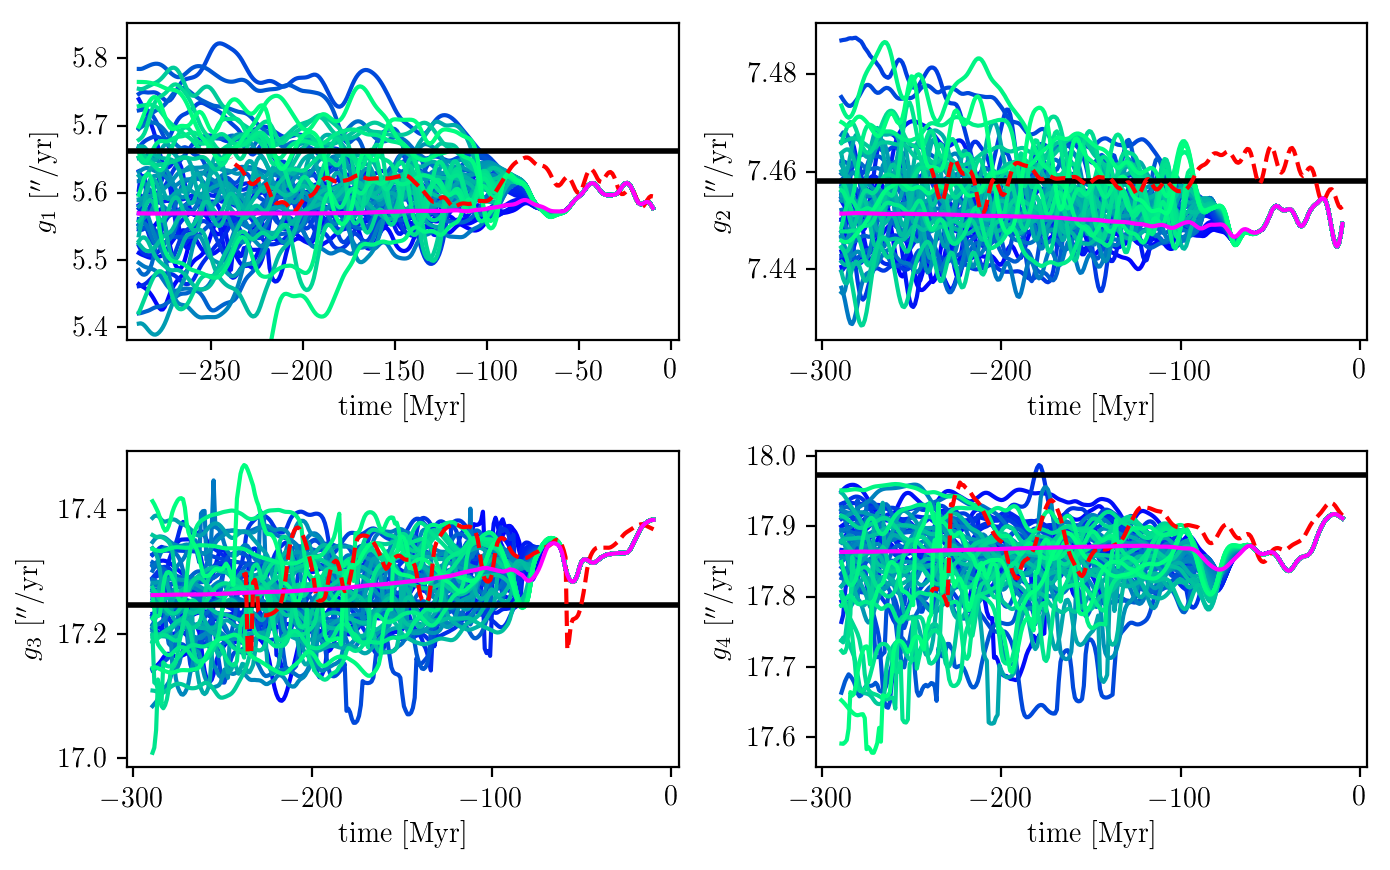
\includegraphics[width=1.0\textwidth,center]{figures/PDF_sample}%
		\caption{Time evolution of: Sample of the first 50 solutions (50 shades of blue), NH frequencies (black horizontal line), La2010d frequencies (red dotted curves) and average of 10,000 solutions (pink curves).}
		\label{fig:sample}
	\end{figure}
	
	\begin{figure} 
		\centering
		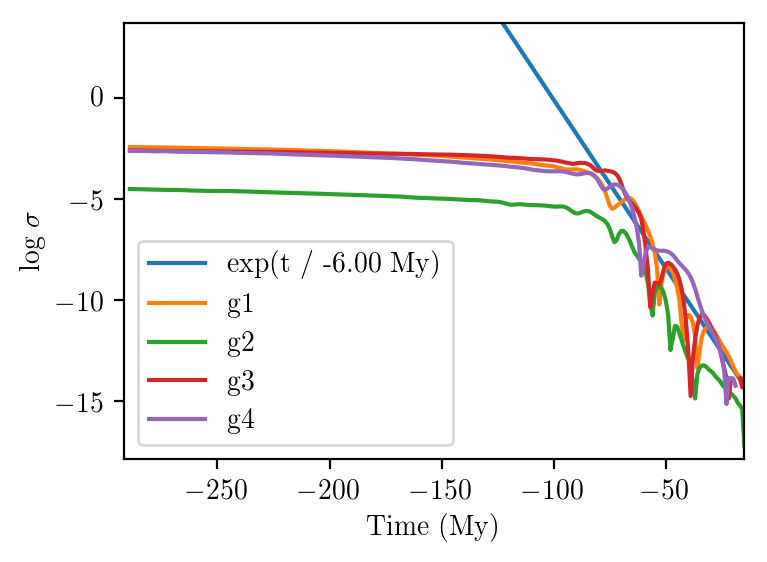
\includegraphics[width=0.5\textwidth]{figures/log_sigma_g2.png}%
		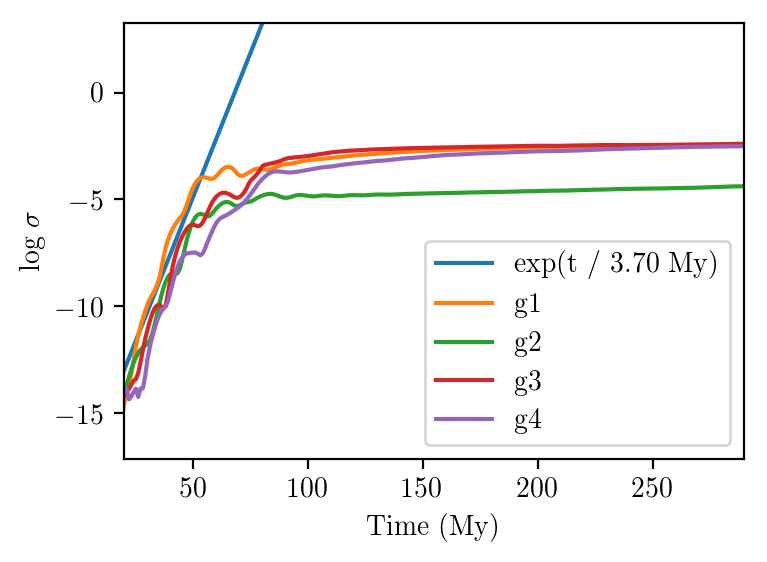
\includegraphics[width=0.5\textwidth]{figures/log_sigma_g_+.png}%
		\caption{Evolution of standard deviation of $g_1, g_2, g_3, g_4$ in the past (left) and in the future (right).}
		\label{fig:log_variannce}
	\end{figure}
	
	\begin{figure}
		\centering
		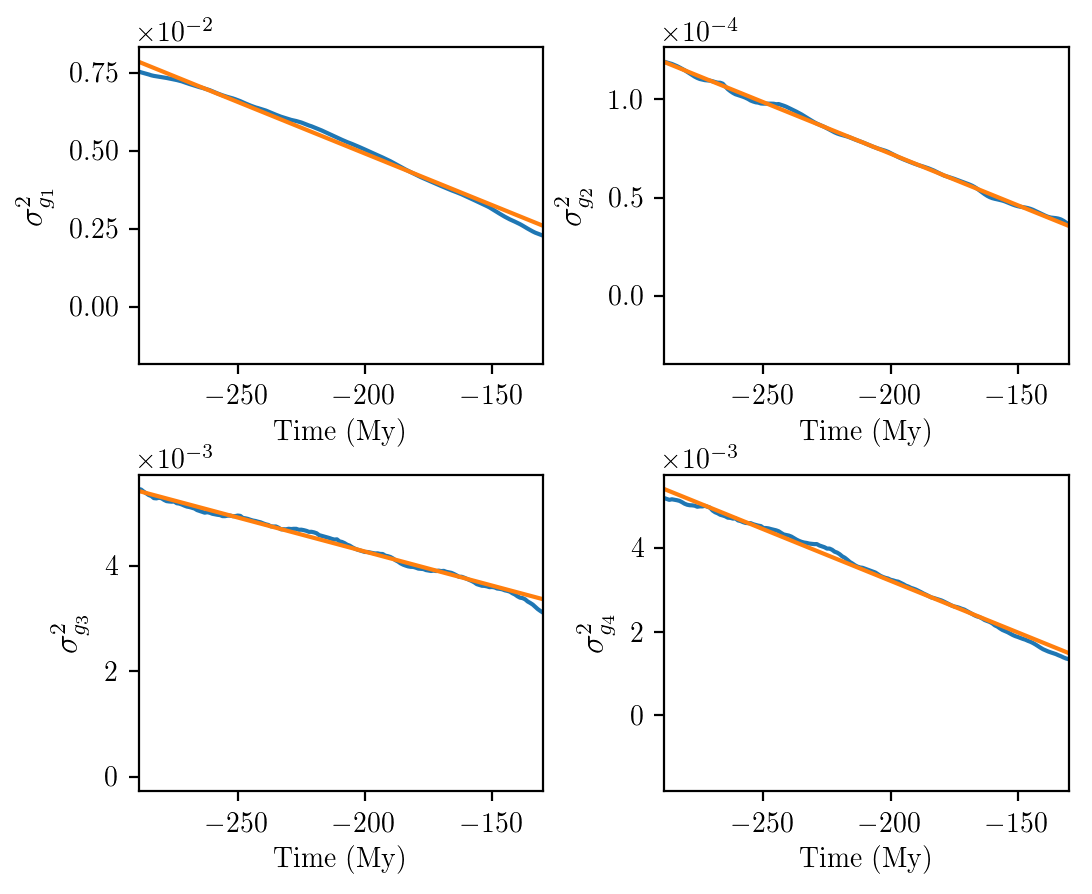
\includegraphics[scale=0.85]{figures/sigma_g2}
		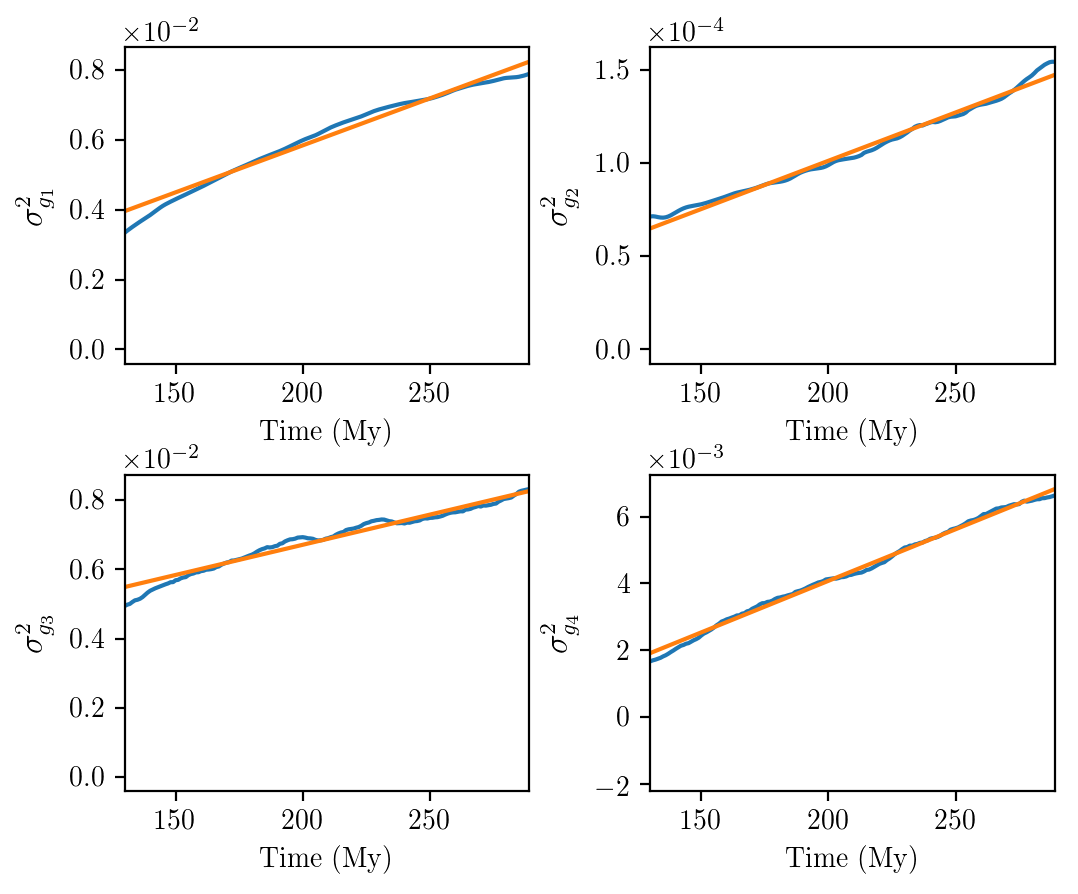
\includegraphics[scale=0.85]{figures/sigma_g_+}
		\caption{Variance of $g_1, g_2, g_3 \text{ and } g_4$ (blue line) and its linear fitting line (orange) whose parameters are described in table \ref{table:sigma2}.  }
		\label{fig:variance}
	\end{figure}
	
	
	\begin{figure}
		\centering
		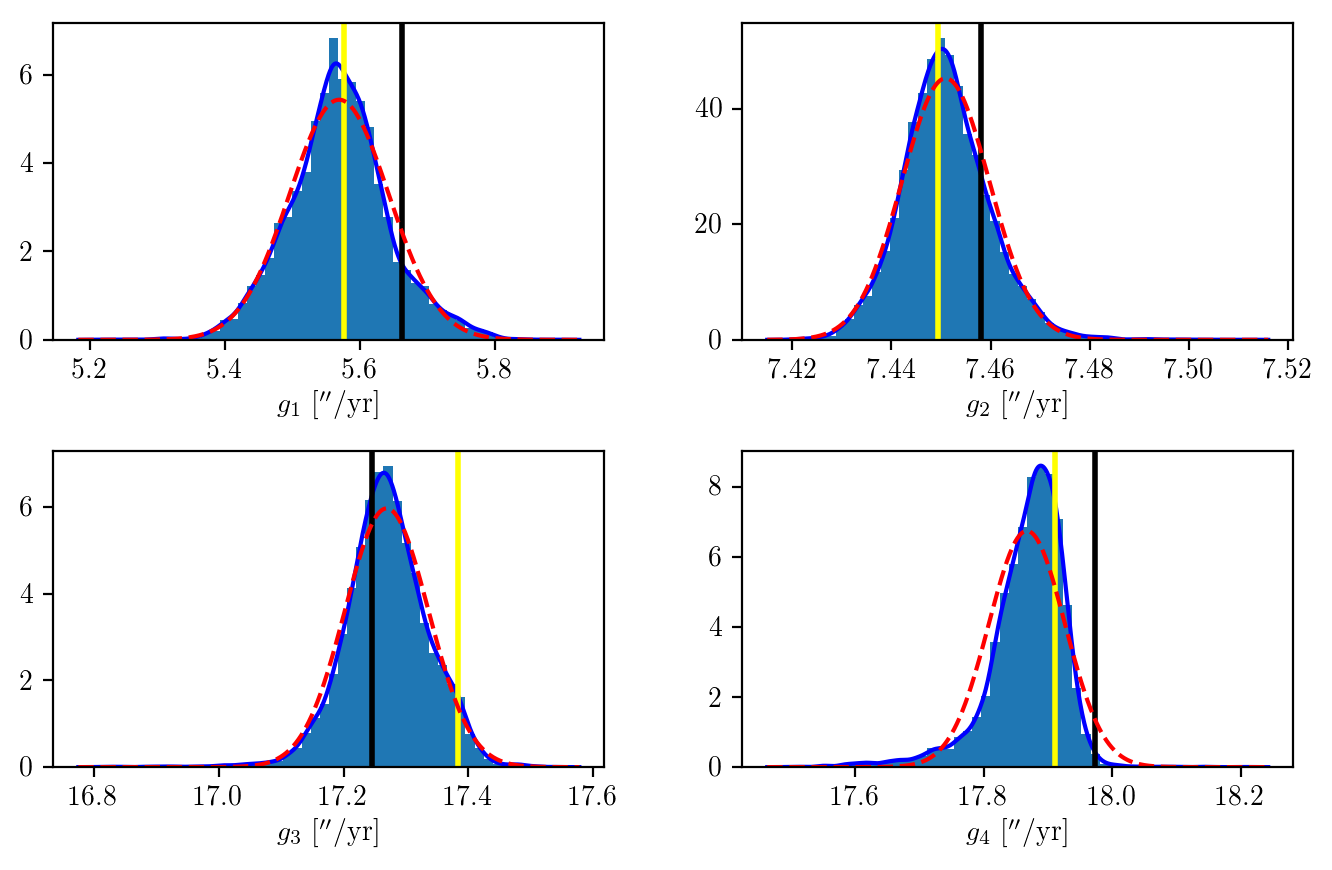
\includegraphics[scale=0.85,center]{figures/PDF_g_210g}
		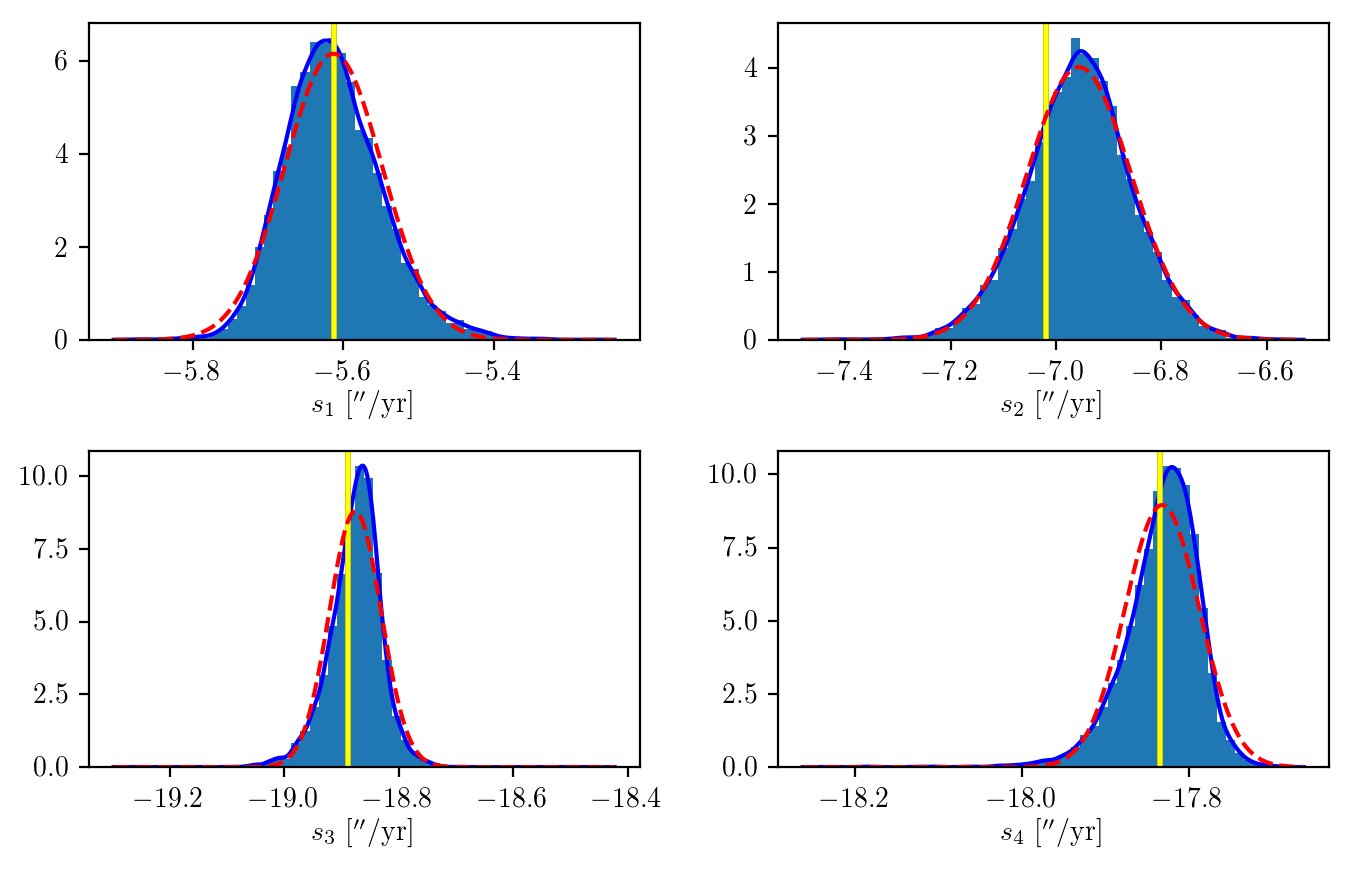
\includegraphics[scale=0.85,center]{figures/PDF_s_210g}    
		\caption{PDF of the fundamental frequencies computed from data of interval [-200 Myr, -220 Myr] in blue. Red curves are the Gaussian functions with the same means and variances, black vertical lines are NH frequencies, yellow vertical lines are current values.}
		\label{fig:past}
	\end{figure}
	
	\begin{figure}
		\centering
		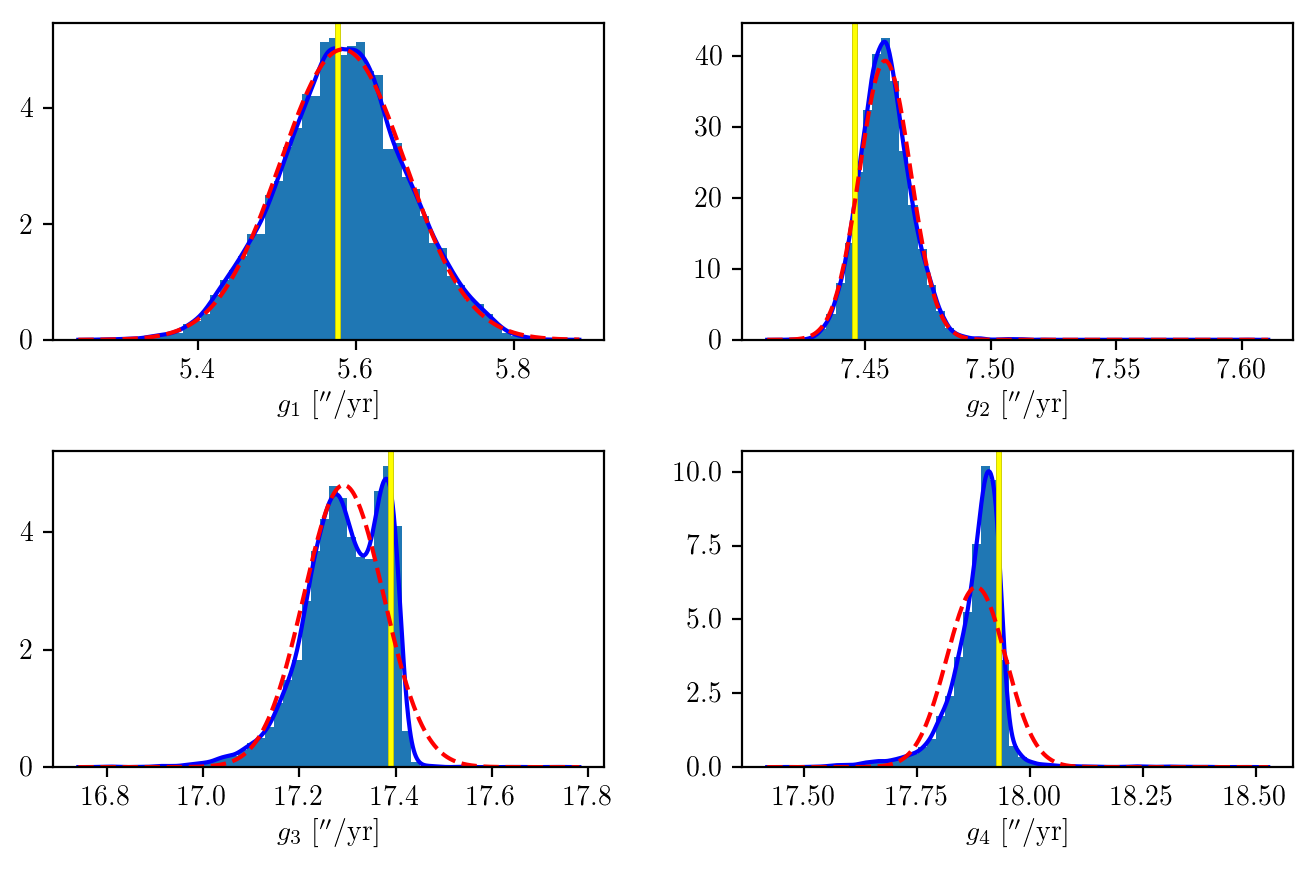
\includegraphics[scale=0.85,center]{figures/PDF_g_210_+}
		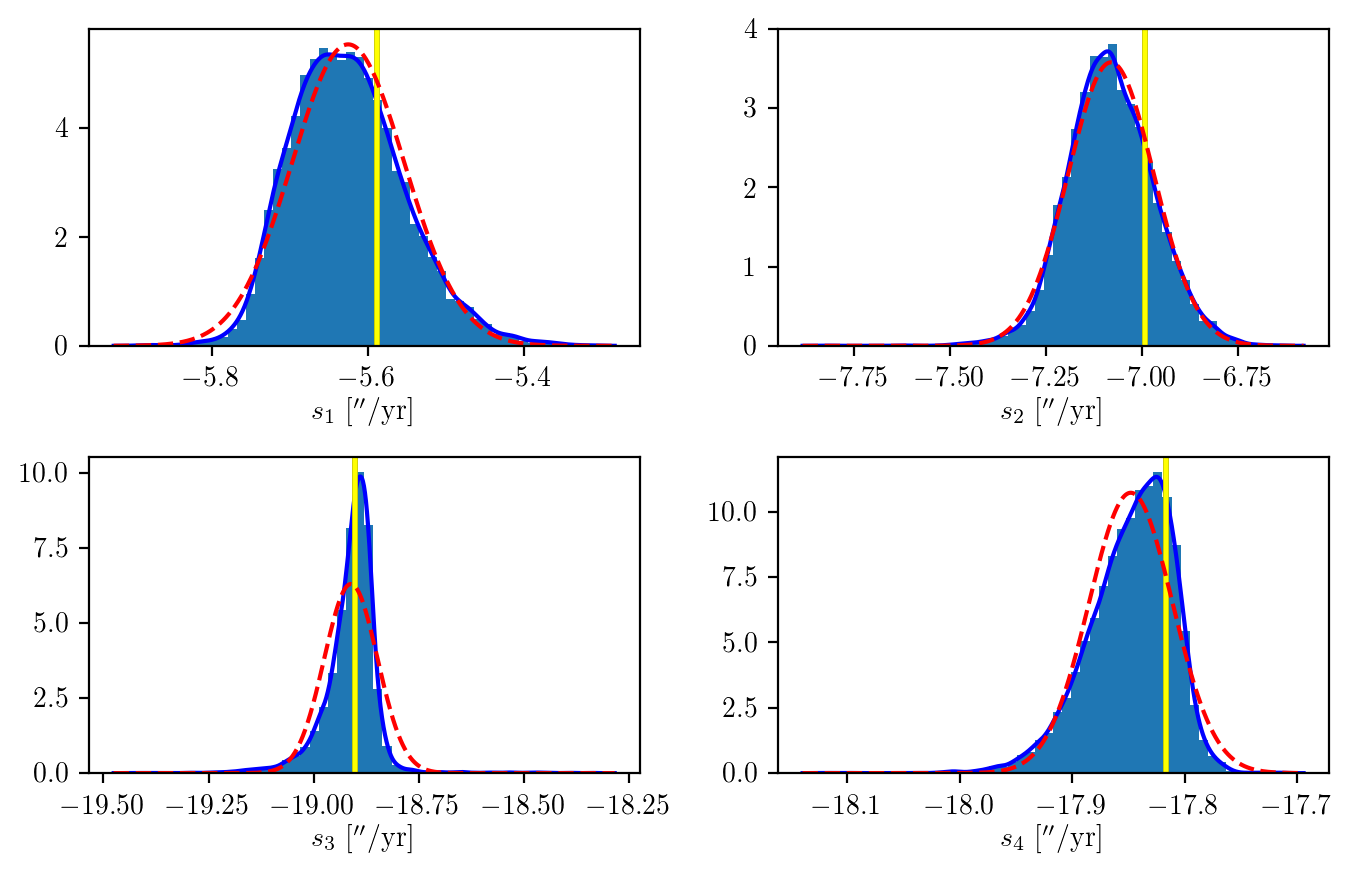
\includegraphics[scale=0.85,center]{figures/PDF_s_210_+}    
		\caption{PDF of the fundamental frequencies computed from data of interval [+200 Myr, +220 Myr] in blue. Red curves are the Gaussian functions with the same means and variances, yellow vertical lines are current values.}
		\label{fig:future}
	\end{figure}
	The evolution of the fundamental frequencies of 50 sample solutions is shown in Fig. \ref{fig:sample}. From 0 to 50 Myr, 50 solutions practically followed the same path; the differences are imperceptible. 
	The La2010d solution is also shown here to compare. While initially, the La2010d frequencies are very close to those of the ensemble, they follow different paths very soon after, this is due to their different Hamiltonians. At around $\pm 60 $ Myr, the frequencies of the ensemble diverge from each other, which makes it impossible to determine the exact path that the actual system has taken.
	A more quantitative view of this divergence is shown in Fig. \ref{fig:log_variannce}. The standard deviations of all the frequencies grow exponentially with a rate of 1/6 $\text{Myr}^{-1}$ in the past, 1/3.7  $\text{Myr}^{-1}$ in the future. The asymmetry between the two directions is apparent from the beginning, the future is interestingly more chaotic than the past.
	At around -100 Myr, the difference between the solutions reach the effective size of phase space, which limits the growth. Beyond -100 Myr, the solutions wander randomly in their immediate phase space and their frequencies undergo a so-called chaotic diffusion. Their means stay relatively constant and their variances increase linearly with time, which is shown in Fig. \ref{fig:variance}.  The coefficients of this linear evolution are written in table (\ref{table:sigma2}).
	
	\begin{table}[ht]
		\centering
		
		\begin{tabular}[t]{ccccc}
			\toprule
			Frequencies & $a_p$ $[''/yr]^2$ & $b_p$ $[''/yr]^2 \text{Myr}^{-1}$   & $a_f$ $[''/yr]^2$ & $b_p$ $[''/yr]^2 \text{Myr}^{-1}$\\
			\midrule
			$g_1$& $-1.69 \times 10^{-3}$ & $-3.30 \times 10^{-5}$ & $4.64 \times 10^{-4}$ & $ 2.69 \times 10^{-5}$\\
			$g_2$& $-3.22  \times 10^{-5}$ &$-5.23 \times 10^{-7}$ & $-2.35 \times 10^{-6}$ & $ 5.19 \times 10^{-7}$\\
			$g_3$& $+1.69 \times 10^{-3}$ & $-1.29 \times 10^{-5}$ & $3.22 \times 10^{-3}$ & $ 1.75 \times 10^{-5}$\\
			$g_4$& $-1.71 \times 10^{-3}$ & $-2.47 \times 10^{-5}$ & $-2.11 \times 10^{-3}$ & $3.09 \times 10^{-5}$\\        
			%            $s_1$& 0 & 2\\
			%            $s_2$& 1 & 3\\
			%            $s_3$& 0 & 2\\
			%            $s_4$& 1 & 3\\        
			\bottomrule
		\end{tabular}
		\caption{Coefficients characterising the chaotic diffusion of the frequencies: $\sigma^2 = a_{p,f} + bT_{p,f}$, where $T$ is time [Myr], $p$ and $f$ denote past and future respectively.}
		\label{table:sigma2}
	\end{table}
	
	Figure (\ref{fig:past} - \ref{fig:future})  show the probability density functions (PDF) of all the fundamental frequencies centered at -210 Myr and +210 Myr. It should be noticed that the initial PDF is a delta function of values in table (\ref{table:ini}). The frequencies PDF randomized by the chaos; beyond -100 Myr, they have effectively ``forgotten" about their initial distribution, and followed a stochastic process. 
	While the PDF of each frequency in the past and in the future are mostly similar, several differences are visible, especially for the PDF of $g_3$ in the future, which contain two adjacent distinct peaks. The PDF could be roughly approximated by Gaussian functions with constant means and linearly-increasing variances. 
	
	It's also interesting to see whether the frequencies could be treated as independent random variables as in the case of integrable system. To do this, we compute the Pearson correlation coefficient. A Pearson correlation coefficient between $x$ and $y$ is defined as:
	\begin{equation}
	r_{x,y} = \frac{\text{cov}(x, y)}{\sigma_x \sigma_y},
	\end{equation}
	where cov is the covariance, $\sigma_x$ and $\sigma_y$ are standard deviation of $x$ and $y$. The coefficient ranges from -1 to 1, where 1 (or -1) describe a perfect positive (or negative) linear relationship, 0 means that there's no correlation.  The table (\ref{table:pearson}) of Pearson coefficients show non-negligible correlations between frequencies, which indicate that they are not independent as predicted in the linear theory. The correlation is especially strong between those who are involved in the same resonance, between ($g_3, g_4, s_3, s_4$) in ($\theta_1, \theta_2$) for example. 
	\begin{table}[ht]
		\centering
		\begin{tabular}{lllllllll}
			\toprule
			{} &   $g_1$ &   $g_2$ &   $g_3$ &   $g_4$ &   $s_1$ &   $s_2$ &   $s_3$ &   $s_4$ \\
			\midrule
			$g_1$ &   1.000 &   0.194 &  -0.438 &  -0.621 &   0.119 &  -0.022 &  -0.377 &  -0.303 \\
			$g_2$ &   0.194 &   1.000 &  -0.074 &  -0.173 &  -0.596 &  -0.325 &  -0.262 &  -0.160 \\
			$g_3$ &  -0.438 &  -0.074 &   1.000 &   0.507 &  -0.086 &   0.034 &   0.022 &   0.071 \\
			$g_4$ &  -0.621 &  -0.173 &   0.507 &   1.000 &  -0.151 &   0.041 &   0.074 &   0.187 \\
			$s_1$ &   0.119 &  -0.596 &  -0.086 &  -0.151 &   1.000 &   0.305 &  -0.098 &  -0.079 \\
			$s_2$ &  -0.022 &  -0.325 &   0.034 &   0.041 &   0.305 &   1.000 &   0.035 &   0.002 \\
			$s_3$ &  -0.377 &  -0.262 &   0.022 &   0.074 &  -0.098 &   0.035 &   1.000 &   0.641 \\
			$s_4$ &  -0.303 &  -0.160 &   0.071 &   0.187 &  -0.079 &   0.002 &   0.641 &   1.000 \\
			\bottomrule
		\end{tabular}
		\caption{Pearson coefficients of the fundamental frequencies at 300 Myr.}
		\label{table:pearson}
	\end{table}
	
	
	
	\subsection{Discussion} \label{sec:dis_den}
	\begin{figure}
		\centering
		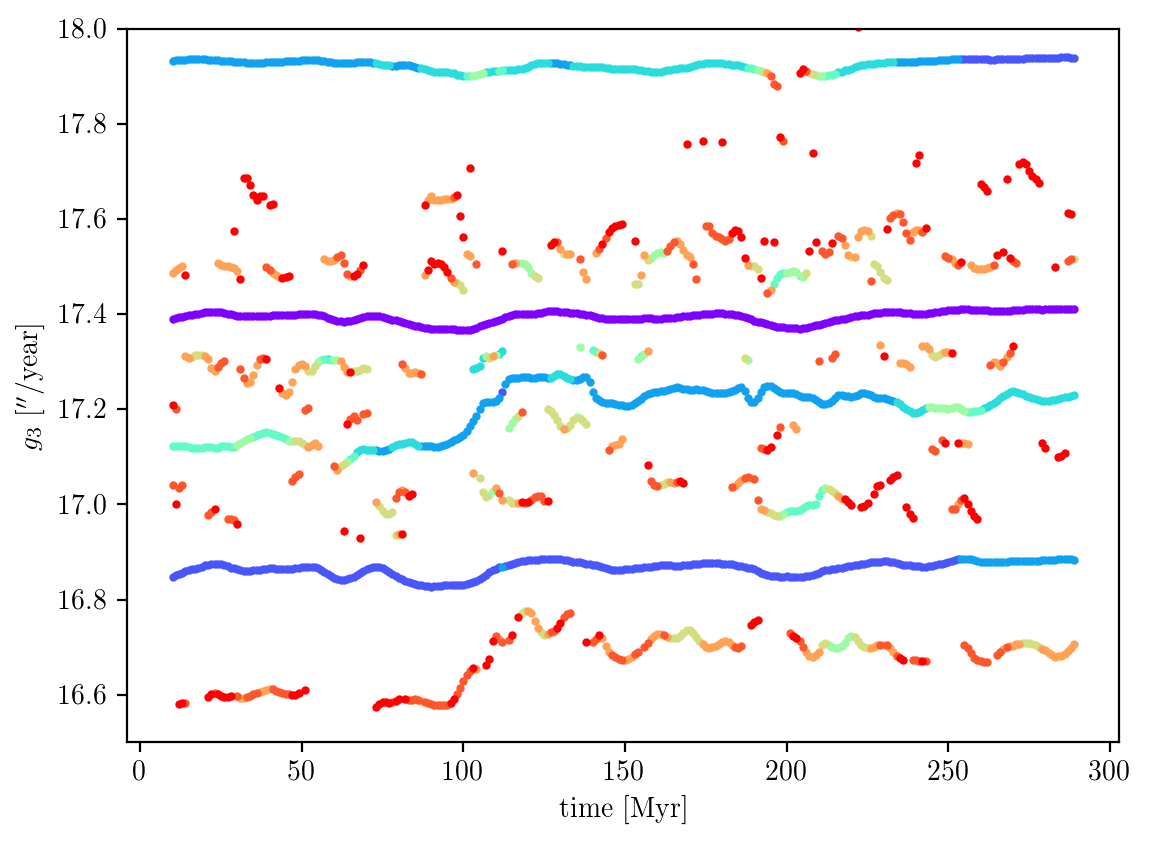
\includegraphics[scale=0.55]{figures/g3_cont_1398+}%
		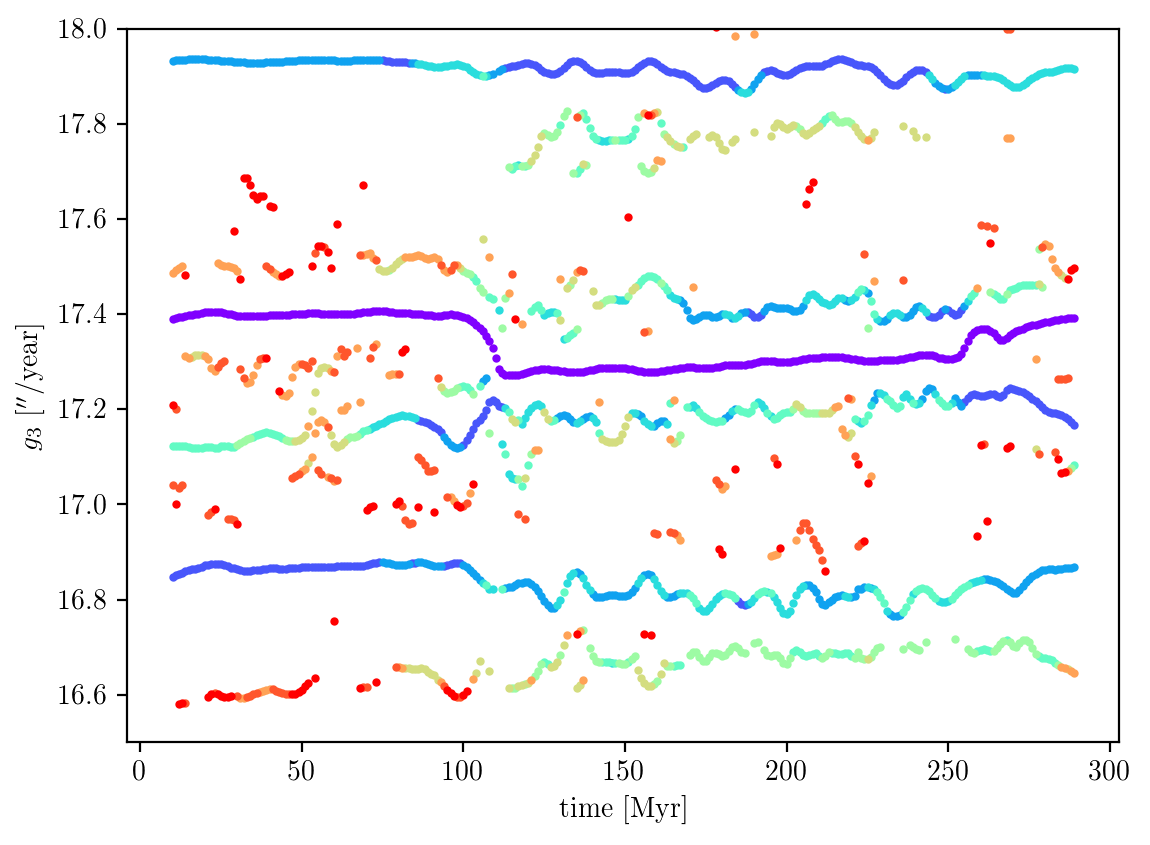
\includegraphics[scale=0.55]{figures/g3_cont_1401b+}%
		\caption{Two different cases of the evolution of $g_3$. Violet indicates a strong mode while red indicates a weak mode, the shade of color in the middle indicate their strength accordingly. }
		\label{fig:g_3_+}
	\end{figure}
	The PDF could be generally approximated by Gaussian functions. This is different from the Rice distribution describing the evolution of eccentricities that has been reported by \cite{laskar2008}:
	\begin{equation} \label{eq:rice}
	f_R(x)  = \frac{1}{\sqrt{2 \pi \sigma^2}} \exp \left( - \frac{x^2 + m^2}{2 \sigma^2} \right) \sqrt{2\pi} \frac{x}{\sigma}  I_0 \left( \frac{xm}{\sigma^2} \right),
	\end{equation} 
	where $I_0(z)$ is the modified Bessel function of the first kind. The Rice distribution simply describes the distribution of the norm of 2 Gaussian variables, which is the case for eccentricity and inclination, that are always positive. Therefore it is consistent with our results.
%	This difference could be understood as follows.	 The Rice distribution (Eq. \ref{eq:rice}) is made up of two part: The Gaussian part and the complementary sinusoidal part, which together represent two different processes. The Gaussian part depicts the long-term chaotic diffusion of the frequencies; the complementary  part, on the other hand, describes the short-term regular quasi-periodic motion of the eccentricity; hence we have the Rice distribution in the actual numerical simulations. A demonstration of this simple model was presented by \cite{federico2017}. Nevertheless, as for the fundamental frequencies, they do not oscillate in a quasi-periodic manner like eccentricities, they are rather constant in short time-scale.Therefore, their distributions follow only those of a stochastic process, which is usually modeled as a Random Walk, where the variances $\sigma^2$ of the distribution grow linearly with time, which is shown by Fig. \ref{fig:variance}. 
	Nevertheless, the deviation of the actual PDF from the Gaussian distributions is discernible. The PDF of $g_4$ and $s_3$, for example, are actually narrower, and the asymmetry is also visible in many cases. This deviation from a simple random walk process indicates that the resonances ($\theta_1$ and $\theta_2$ in particular) have a strong impact on the dynamics.
	The PDF of $g_3$ at +210 Myr show 2 prominent peaks, which is different from all other PDF. This anomaly is illustrated in Fig. \ref{fig:g_3_+}. It was obtained by analyzing the frequency of the proper variable relating to $g_3$ of 2 different solutions. One frequency, which is normally much stronger than others (in violet), will be assigned for $g_3$; other weaker frequencies in the spectrum will have red-ish color. We discovered that the evolutions of $g_3$ in the future exhibit 2 different scenarios: (1) diffuse around the initial value and (2) being suddenly ``pulled"  toward the lower immediate mode, then settle at a middle value and diffuse normally (Fig. \ref{fig:g_3_+}). Therefore, the PDF of $g_3$ show two adjacent Gaussian functions, which describe 2 diffusion process around 2 mean values.
	
	\section{Geological Constraints from Newark-Hartford data} \label{sec:geo_con}
	
	\begin{table}
		\centering
		\begin{tabular}{cllllll}
			%        \toprule
			{} &   $\epsilon_L$ &   $2\epsilon_L$ &   $4\epsilon_L$ &   $\epsilon_S/4$ &   $\epsilon_S/2$ &   $\epsilon_S$  \\
			\midrule
			$g_1$                &  2244 &  5509 &  9362  &  649 &   1491 &  3629   \\
			$g_3$                 &  1252 &  2452 &  4601  &  2075&   3932 &  6650  \\
			$g_4$                 &  165  &  556  &  2857  &  122 &   369  &  1821    \\
			($g_1, g_3, g_4$)   &  0    &  5    &  733   &  0   &   2    &  31   \\
			\midrule
			$g_1$                &  3502 &  6979 &  9694  &  1557 &   2577 &  5114   \\
			$g_3$                 &  4281 &  5426 &  7221  &  5105 &   6700 &  8533 \\
			$g_4$                 &  411  &  1138 &  4333  &  343  &   197  &  2996    \\
			($g_1, g_3, g_4$)   &  7    &  68    &  2090  &  0   &   11   &  182   \\
			\bottomrule
		\end{tabular}
		\caption{Number of solutions whose difference between their frequency and NH frequency smaller than $\epsilon_L$ and $\epsilon_S$ centered at -210 Myr (top), and centered over the range [-200 Myr; -225 Myr] (bottom). $\epsilon_L$ is the absolute difference between the frequencies of La200d and NH frequencies; $\epsilon_S$ is the standard deviation of the PDF of each frequency.}
		\label{table:epsilon}
	\end{table}
	\begin{figure}[t]
		\centering
		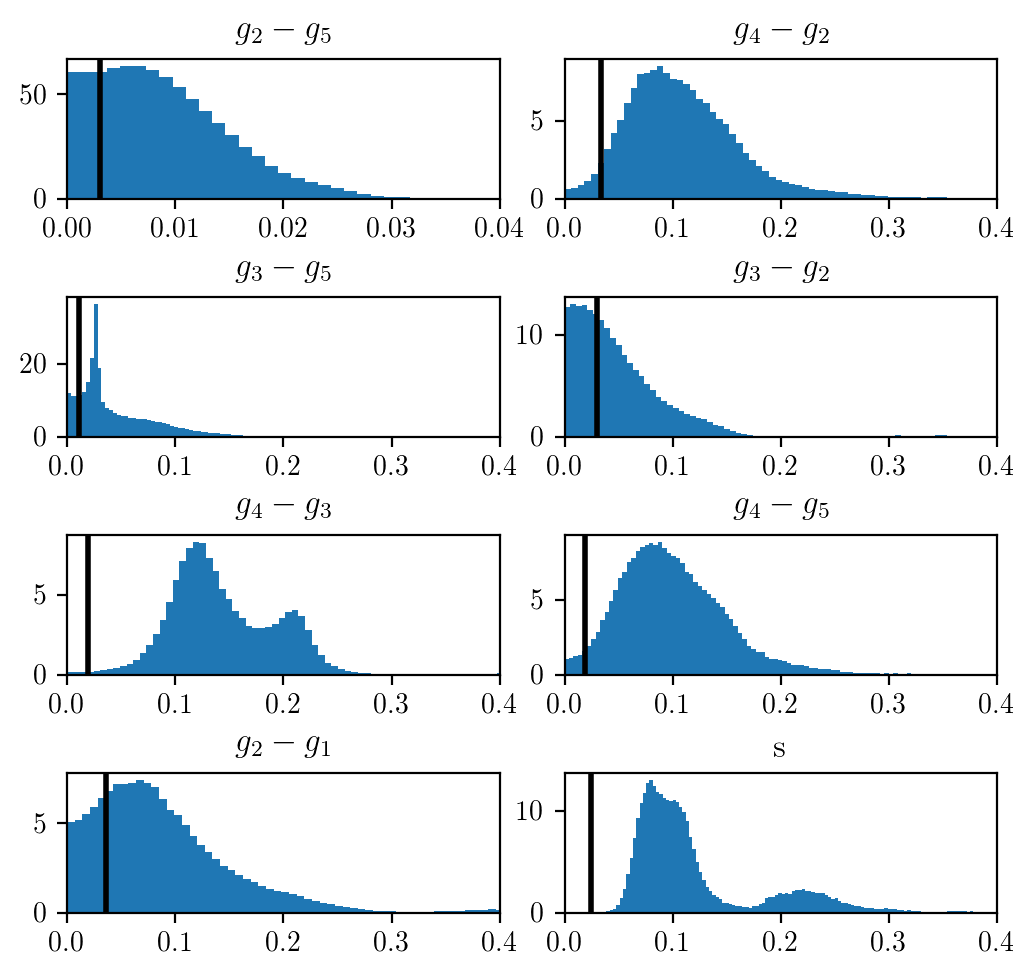
\includegraphics[scale=1.0]{figures/PDF_ecc_all3}
		%        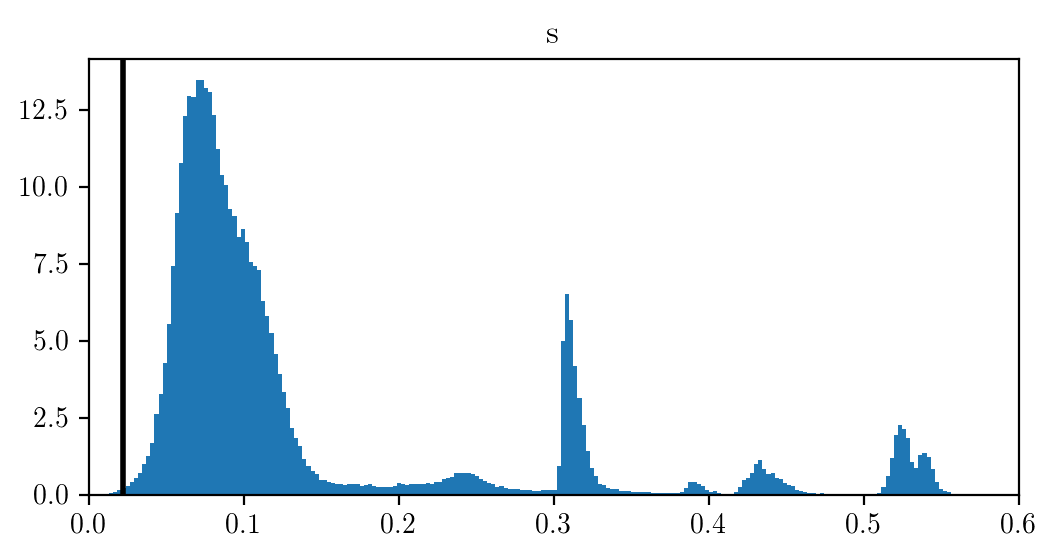
\includegraphics[height=0.3\textheight,width=0.95\textwidth]{figures/PDF_ecc_s_avec}    
		\caption{PDF of the absolute difference of main frequencies ($''$/yr) between Earth's eccentricity and the NH data (blue), their averaged value s (Eq. \ref{eq:s}) (right bottom), and between those of La2010d and NH data (black vertical lines). }
		\label{fig:PDF_ecc}
	\end{figure}    
	
	The fundamental frequencies obtained from the geological record \citep{olsen2019} are done in the following way. The data was dated by the relatively stable 405-kyr McLaughlin cycle ($g_2 - g_5$), and additionally verified by other timing methods. Then, a frequency analysis (Sect. \ref{sect:FA}) was performed on the geological data as well as the eccentricity of astronomical solution (La2010d) to retrieve their strongest frequencies. They PDF later cross-checked with each other to identify its orbital counterpart. For example, the third strongest frequency 12.989 $[''/ yr]$ from Newark data is identified with the second strongest frequency 12.978 $[''/ yr]$ from La2010d, which is $g_3- g_5$. To obtain $g_3$, they just needed to take the sum of this $g_3- g_5$ and $g_5$, which is almost constant. The same went for $g_1, g_2$ and $g_4$. Definite values of astronomical fundamental frequencies PDF thus determined. Nevertheless, it is still very difficult to evaluate the uncertainty of each frequency. We are therefore obliged to define it here ourselves. 
	\begin{table}[t]
		\begin{tabular}{ccccccccc}
			\hline
			
			{}                     & Freq [$"$/yr]           & Amp                & Freq [$"$/yr]          & Amp                    & Freq [$"$/yr]                   & Amp                    & Freq [$"$/yr]         & Amp                    \\
			{}              & \multicolumn{2}{c}{NH}            & \multicolumn{2}{c}{La2010d}                         & \multicolumn{2}{c}{Mo19a}                         & \multicolumn{2}{c}{Mo19b}                        
			\\ \hline
			
			1 & \textbf{3.200} & 1.000 & \textbf{3.203} & 1.000 & \textbf{3.192} & 1.000 & \textbf{3.194} & 1.000 \\
			2 & \textbf{12.989} & 0.437 & \textbf{12.980} & 0.701 & \textbf{13.710} & 0.533 & \textbf{13.010} & 0.584 \\
			3 & \textbf{10.530} & 0.406 & \textbf{9.778} & 0.548 & \textbf{13.010} & 0.526 & \textbf{13.730} & 0.577 \\
			4 &  \textbf{0.742} & 0.349  & \textbf{13.690} & 0.333 & \textbf{9.806} & 0.487 & \textbf{9.788} & 0.557 \\
			5 & \textbf{9.806} & 0.341   & 13.850 & 0.274 & \textbf{10.530} & 0.365 & \textbf{10.540} & 0.416 \\
			6 & \textbf{13.716} & 0.340 & \textbf{10.490} & 0.244 & \textbf{0.735} & 0.241 & \textbf{0.748} & 0.284 \\
			7 &  10.670 			& 0.333& 13.990 & 0.236 & 1.305 & 0.217 & 1.355 & 0.265 \\
			8 & 17.106 & 0.245 & \textbf{0.721} & 0.232 & 12.960 & 0.191 & \textbf{1.822} & 0.181 \\
			9 & 13.427 & 0.245 & 1.351 & 0.230 & \textbf{1.886} & 0.166 & 13.880 & 0.162 \\
			10 & 57.274 & 0.223  & 13.760 & 0.221 & 10.430 & 0.150 & 13.470 & 0.162 \\
			11 & 2.457 & 0.210& 10.280 & 0.215 & 13.810 & 0.136 & 13.610 & 0.156 \\
			12 &\textbf{1.802} & 0.207  & 10.780 & 0.206 & 13.620 & 0.128 & 0.573 & 0.153 \\
			13 &   12.189 & 0.206 & 13.440 & 0.199 & 2.665 & 0.125 & 10.380 & 0.153 \\
			14 &  9.911 & 0.204& 10.650 & 0.193 & 10.940 & 0.120 & 11.630 & 0.152 \\
			15 &  &  & 10.420 & 0.190 & 0.369 & 0.119 & 12.960 & 0.120 \\
			16 &  &  & 0.494 & 0.188 & 12.980 & 0.110 & 14.150 & 0.100 \\
			17 &  &  & \textbf{1.883} & 0.178 & 13.080 & 0.109 & 23.550 & 0.093 \\
			18 &  &  & 13.280 & 0.135 & 12.980 & 0.100 & 16.180 & 0.079 \\
			19 &  &  & 0.614 & 0.127 & 12.930 & 0.098 & 2.453 & 0.077 \\
			20 &  &  & 11.620 & 0.127 & 13.400 & 0.097 & 12.950 & 0.059 \\
			{$s$}              & \multicolumn{2}{c}{0}            & \multicolumn{2}{c}{0.025}                         & \multicolumn{2}{c}{0.033}                         & \multicolumn{2}{c}{0.015}                        \\
			{$s'$}              & \multicolumn{2}{c}{0}            & \multicolumn{2}{c}{0.022}                         & \multicolumn{2}{c}{0.010}                         & \multicolumn{2}{c}{0.014}                        \\
			\hline
		\end{tabular} 
		\caption{The strongest frequencies and their normalized amplitudes of NH data, La2010d and our best solutions: with smallest $s$ (Fe19b) and smallest $s'$ (Fe19a). Bold frequencies are the selected frequencies (detailed in table \ref{table:f_compare}).}
		\label{table:fa_compare}
	\end{table}
	Fig. \ref{fig:past} shows how chaotic diffusion can bring fundamental frequencies away from initial value to NH frequencies centered at -210 Myr. $g_1, g_2$ and $g_3$ of NH data lie completely inside the bulge of PDF; $g_4$ however is at the tail, therefore, a solution that actually went there is quite unlikely. The standard deviations of $g_1, g_3, g_4$ are of $\sim$ 0.1 $''$/yr, $g_2$, on the contrary, vary 10 times less, of around $\sim$  0.01 $''$/yr. This result validates the exceptional stability of the $g_2 - g_5$ Mclaughlin cycle, which \cite{olsen2019} use to date the NH data.
	
	We take La2010d as a standard measure to define how good our solutions are; a solution is considered ``good" when its frequencies are closer to the geological frequencies than those of La2010d. Table \ref{table:epsilon} show how many of such good solutions among our 10,000 solutions. We first considered the frequencies centered at -210 Myr, which means they PDF extracted from data over the interval of [-200 Myr; -220 Myr]. This interval is similar to the interval of the NH data [-200.65 Myr; - 225.565 Myr]. Although $g_1$ and $g_3$ exhibit a decent chance of being ``good", we found no solution that is better than La2010d, which was due to the very low probability ($\sim$ 1.5 $\%$) of finding a solution with good $g_4$. $g_2$ is not considered here because it is already extremely close to that of NH data in most of the cases. Even when doubling the limit (2$\epsilon_L$), we found only 5 solutions whose frequency is this range.
	
	The centers of intervals of orbital solutions, where we extract the frequencies, are then relaxed; they would not be taken like the precise interval of NH data, but are rather displaced  within maximum 10 Myr from the interval of geological data: from [-190 Myr; -210 Myr] until [-215 Myr; -235 Myr]. The length of intervals  (20 Myr) remain unchanged. This flexibility is in accordance with the comparison in \citep{olsen2019}, where the interval of astronomical frequency was taken to be [-209 Myr; -231 Myr], which was around 9 Myr different from the NH interval. The averaged PDF of the frequencies over the displacing range are very close to those centered at -210 Myr (Fig. \ref{fig:past}), and will then be shown here. With these relaxed intervals, we found more solutions that are close to the NH data, in particular, 7 ``good" solutions are better than La2010d.
	
		\begin{table}[t]
		\centering
		\begin{tabular}[t]{ccccc}
			\toprule
			Frequencies & NH FA&  La2010d & Mo19a & Mo19b\\
			\midrule
			$g_2 - g_5$& 3.20 & 3.20 & 3.192 & 3.194 \\
			$g_4 - g_2$& 10.53 & 10.496 & 10.527 & 10.540\\
			$g_3 - g_5$& 12.989 & 12.978 &13.006 & 13.010\\
			$g_3 - g_2$& 9.806 & 9.776 & 9.806 & 9.788\\        
			$g_4 - g_3$& 0.742 & 0.726 & 0.735 & 0.748\\    
			$g_4 - g_5$& 13.716 & 13.697 &13.714 & 13.730\\        
			$g_2 - g_1$& 1.802 & 1.838 & 1.886 & 1.822\\    
			
			$g_1^*$& 5.661 & 5.611 &  5.563 & 5.629 \\
			$g_2^*$& 7.458 & 7.461 & 7.449 & 7.451\\
			$g_3^*$& 17.246 & 17.236 & 17.263& 17.267 \\
			$g_4^*$& 17.973 & 17.955 & 17.971& 13.987\\        
			%Mo19a is 3340
			\bottomrule
		\end{tabular}
		\caption{ 7 selected frequencies. $g_i^*$ are obtained from $g_i - g_5$. }
		\label{table:f_compare}
	\end{table}
	All frequencies analysis above has been done with proper variables (Sect. \ref{sec:det_freq}) to extract the fundamental frequencies. Although this is a convenient and precise way to determine frequencies, the eccentricity of the Earth should be analyzed to give a 1-to-1 comparison with the NH data, because after all, eccentricity was the one who modulated the variation of geological data on Earth. We performed the frequency analysis on Earth's eccentricities over the relaxed intervals from our ensemble of solutions to obtain 20 strongest frequencies for each solution. Among the strongest 10 of each orbital solution, 6 frequencies, that are closest to the 6 pre-selected frequencies (presented in table (\ref{table:f_compare}); they are are also among the strongest 10 in the NH data), PDF chosen. The $7^{th}$ frequency ($g_2 - g_1$) PDF selected in the same way but among  20 strongest frequencies. The difference between each frequency is defined as $\delta_i = \sqrt{(h_i - k_i)^2}$, where $h_i$ is the NH frequency and $k_i$ is the frequency that is chosen to be closest to $h_i$. While the sum $s$ is defined as : 
	\begin{equation} \label{eq:s}
	s = \sqrt{\sum_{i=1..7}^{} \frac{(h_i-k_i)^2}{7}}.
	\end{equation}
	The PDF of the Earth's eccentricity (Fig. \ref{fig:PDF_ecc}) tell the same story as the PDF of fundamental frequencies (Fig. \ref{fig:past}). While the PDF of combinations involving $g_1, g_2, g_3$ is quite close to the NH frequencies, the combinations involving $g_4$ remain the main obstacle for our solutions to be close the NH data. There are only around $\sim$ 10 solutions whose total difference s smaller than that of La2010d. If we only consider the first 6 frequencies without taking the relatively weak $g_2 - g_1$ into account (the new total difference is defined as $s'$), around 150 are found to be better (have smaller $s'$) than La2010d. Table (\ref{table:fa_compare}) compare our two best solutions, one with smallest $s$ (Mo19b) and one with smallest $s'$ (Mo19a), with La2010d to the NH data. The frequencies of our two solutions are closer to those of NH than La2010d (Table \ref{table:f_compare}). The orders of their amplitudes also resemble that of NH data better than La2010d. 
	
	

	\subsection{Discussion}
	The number of solutions that are as good as La2010d is surprisingly poor, considering the sheer number of solutions that we have. Only around 10 among 10,000 solutions that are actually better than 1 in 11 solutions from \cite{olsen2019}. We speculate discrepancy could probably arise from the difference between the mean of the exact distribution and the mean of secular solutions. Currently, distribution from complete equations is not available to compare. Nevertheless, judging from one particular solution La2010d (Fig. \ref{fig:sample}), the deviation of its  $g_1 \text{ and }g_4$ from the means towards the geological data could already be seen. Although with a less complete averaged system of the equation that has been used here, we believe that the secular solutions could give a realistic statistical description of the full solutions, especially their variances and the forms of distribution.
	
	%    \begin{table}[ht]
	%    \centering
	%    \begin{tabular}{c|lll|lll}
	%        \toprule
	%        {} &   $\epsilon_L$ &   $2\epsilon_L$ &   $4\epsilon_L$ &   $\epsilon_S/4$ &   $\epsilon_S/2$ &   $\epsilon_S$  \\
	%        \midrule
	%        $g_1$ &   2209 &  5472 &  9359 &  624 &   1465 &  3586   \\
	%        $g_3$ &  1269 &  2509 &   4718 &  212 &  4039 &  6831  \\
	%         $g_4$ &  165 &  564 &   2886 &  123 &  37 &   1844    \\
	%         ($g_1, g_3, g_4$) &  0&  2 &  777 &  0 &  2 &  39   \\
	%        \bottomrule
	%    \end{tabular}
	%    \caption{Number of good solutions (with continuity) at -210 Myr}
	%\end{table}
	
	\section{Inversion of modes} \label{sec:inv}
	\begin{figure}[t!]
		\centering
		\begin{subfigure}[t]{0.50\textwidth}
			\centering
			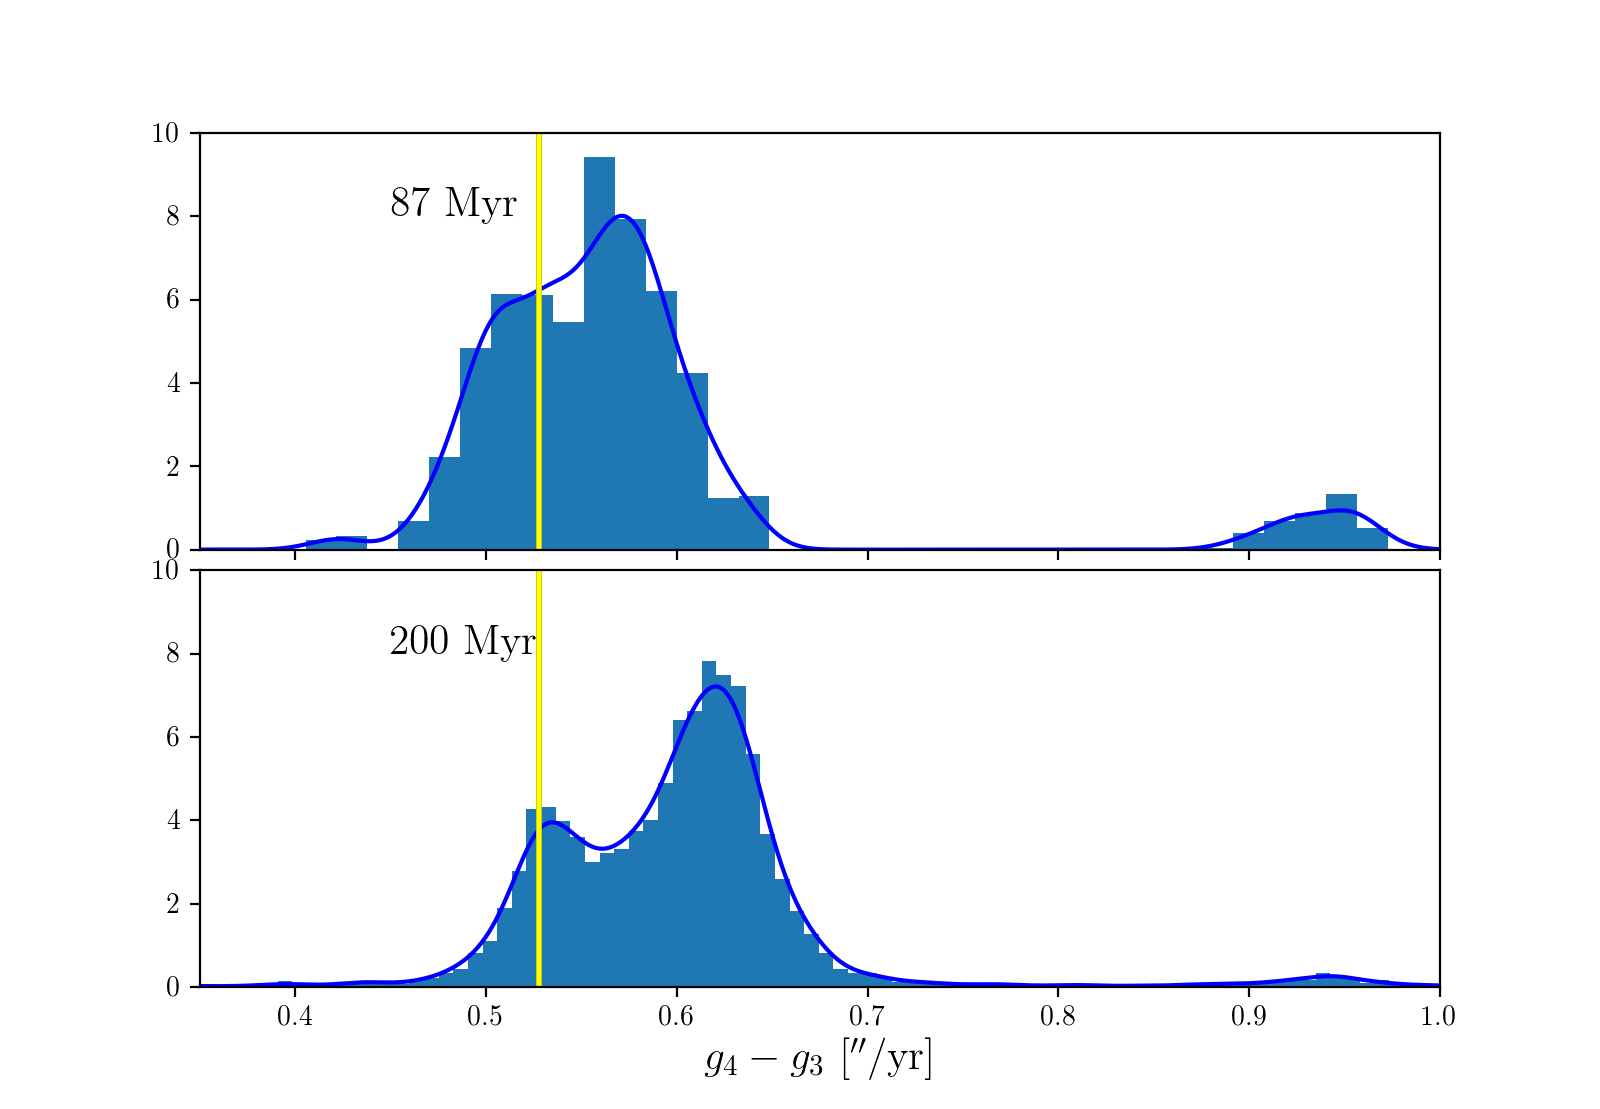
\includegraphics[width=1.0\textwidth,height=0.25\textheight]{figures/PDF_g4g3}%
			\caption{}
			\label{fig:inver_PDFa}
		\end{subfigure}%
		\begin{subfigure}[t]{0.50\textwidth}
			\centering
			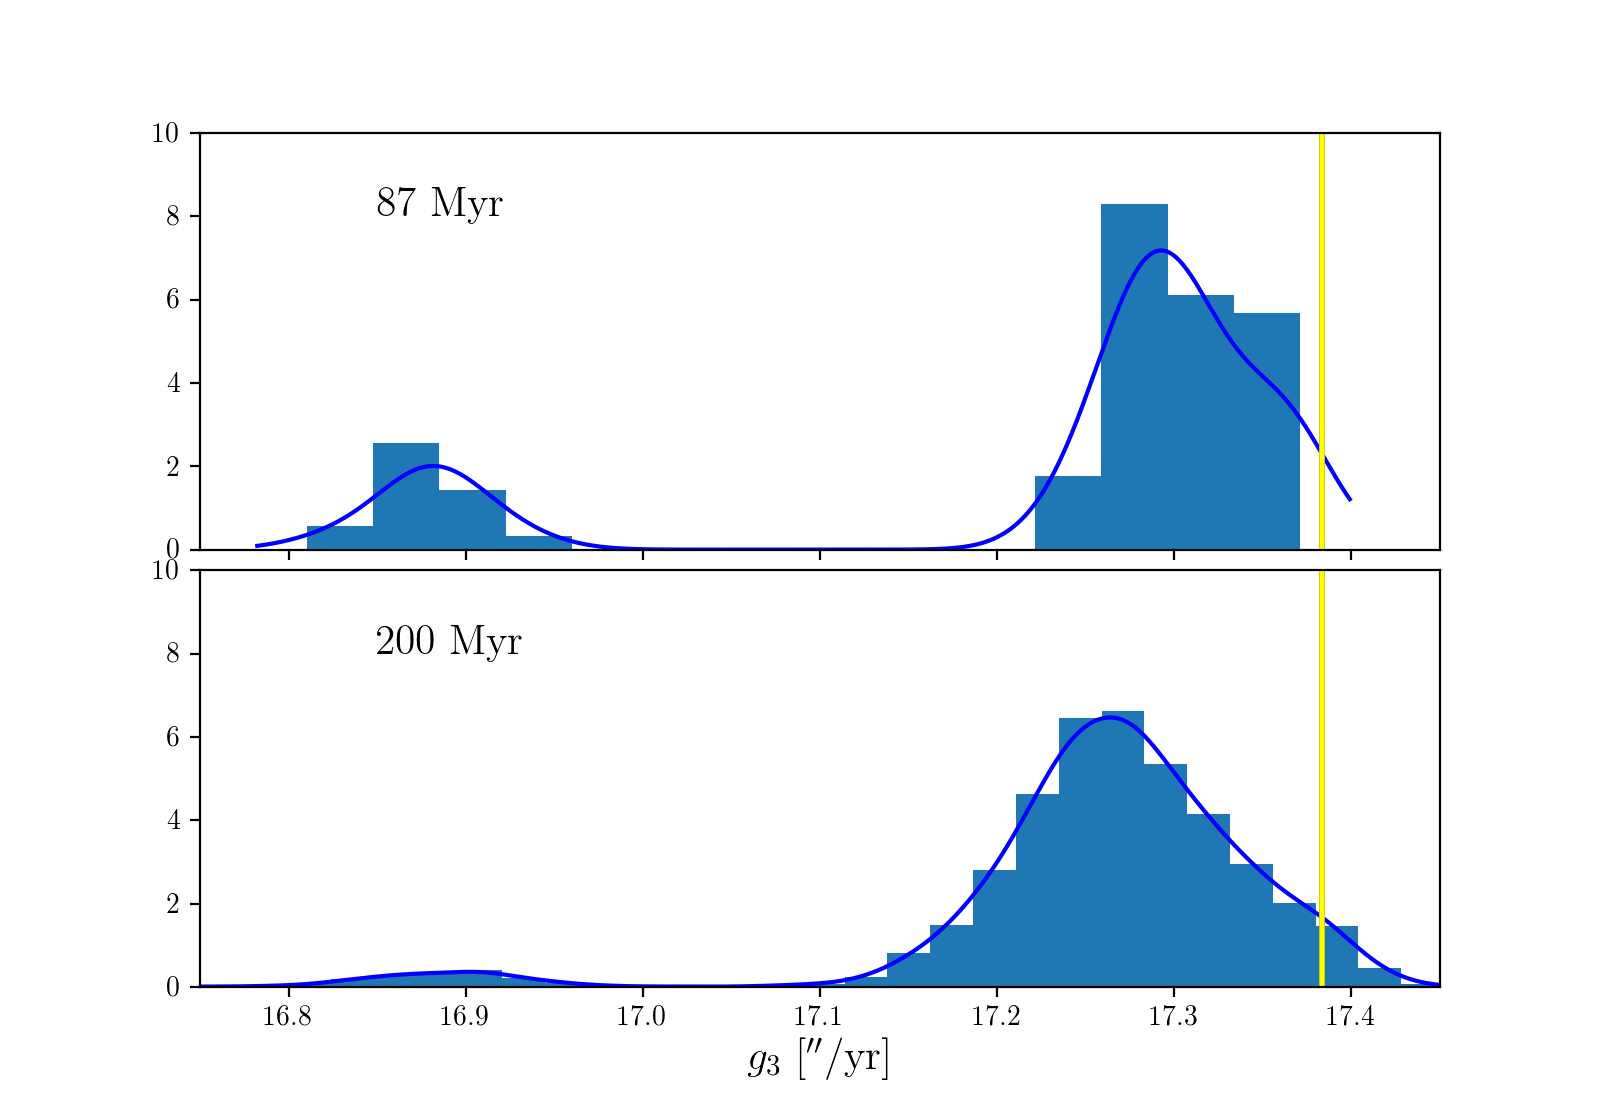
\includegraphics[width=1.0\textwidth,height=0.25\textheight]{figures/PDF_g3_time_big_bin15_50}%
			\caption{}
			\label{fig:inver_PDFb}
		\end{subfigure}
		\caption{PDF of the $g_4-g_3$ (a) and $g_3$ (b). The frequencies PDF obtained by analyzing the data (Earth's eccentricity for $g_4 - g_3$ and proper variable for $g_4$) whose interval of 20 Myr and centered at -87 Myr (top) and -200 Myr (bottom).}
		\label{fig:inver_PDF}
	\end{figure}
	\cite{ma2017} found a sudden change of the period of a long cycle from 2.4 Myr to 1.2 Myr in the Libsack core of Cretaceous basin around [-83 Myr; -90 Myr]. This change was also visible in of La2004 astronomical solution, and the long cycle was attributed to $g_4 - g_3$ from the spectrum of the eccentricity of the Earth. From the band power of their geological data (figure 1 of \cite{ma2017}), the change of the period is visible, but the exact value of the period before and especially after the transition is highly questionable. Therefore, we focus on the transition of $g_4 - g_3$ itself rather than its exact value. To give some estimation, the transition from 2.4 Myr to 1.2 Myr is actually the change of $g_4 - g_3$ from 0.54 ($''$/yr) to 1.08 ($''$/yr). 
	
	From 10,000 secular solutions, we observed a very robust mechanism for this transition. The figure (\ref{fig:inver_PDFa}) shows the PDF of $g_4 - g_3$ around -87 Myr, which is also the time of the transition observed in geological data. This PDF has 2 part: the main part containing 2 peaks, which closely centered around 0.55 ($''$/yr), represent two main density function of $g_4$ and $g_3$ respectively; another smaller part centered at 0.95 ($''$/yr) represent the second peak of $g_3$. This second peak of $g_3$ is visible from the PDF of $g_3$ (Fig. \ref{fig:inver_PDFb}), which is obtained by simply choosing the strongest frequency of the proper variable relating to $g_3$. The second mode centered at 16.9 ($''$/yr), albeit smaller than the principal mode, is quite significant; it accounts for $\sim 10 \% $ of the PDF. Therefore, the transition report by \cite{ma2017} could be understood as the inversion of modes: During the transition time (around -87 Myr), $g_3$ jumps from the main mode to the second mode, which makes $g_4 - g_3$ from the spectrum of eccentricity also jump from its main mode to its second mode; the probability of the jump is $\sim 10 \% $. 
	At around -200 Myr, the PDF look nicer because of chaotic mixing; the size of the second mode shrinks, and the probability of the transition is much smaller.   
	\begin{figure}[t]
		\centering
		\begin{subfigure}[t]{0.47\textwidth}
			\centering
			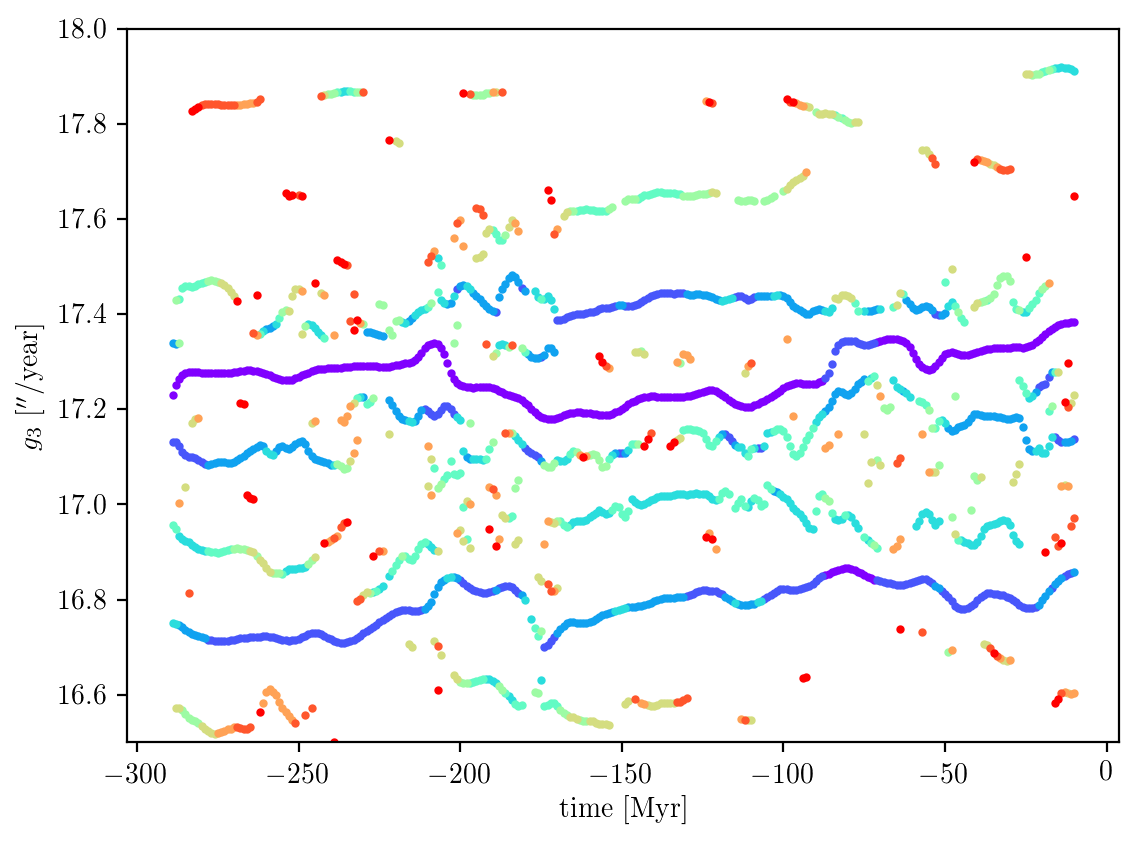
\includegraphics[width=1.0\textwidth]{figures/g3_cont_2944}%
			\caption{The evolution of the modes $g_3$. Violet indicates a strong mode while red indicates a weak mode, the shade of color in the middle indicate their strength accordingly.}
			\label{fig:inv_examplea}
		\end{subfigure}%
		\hfill
		\begin{subfigure}[t]{0.47\textwidth}
			\centering
			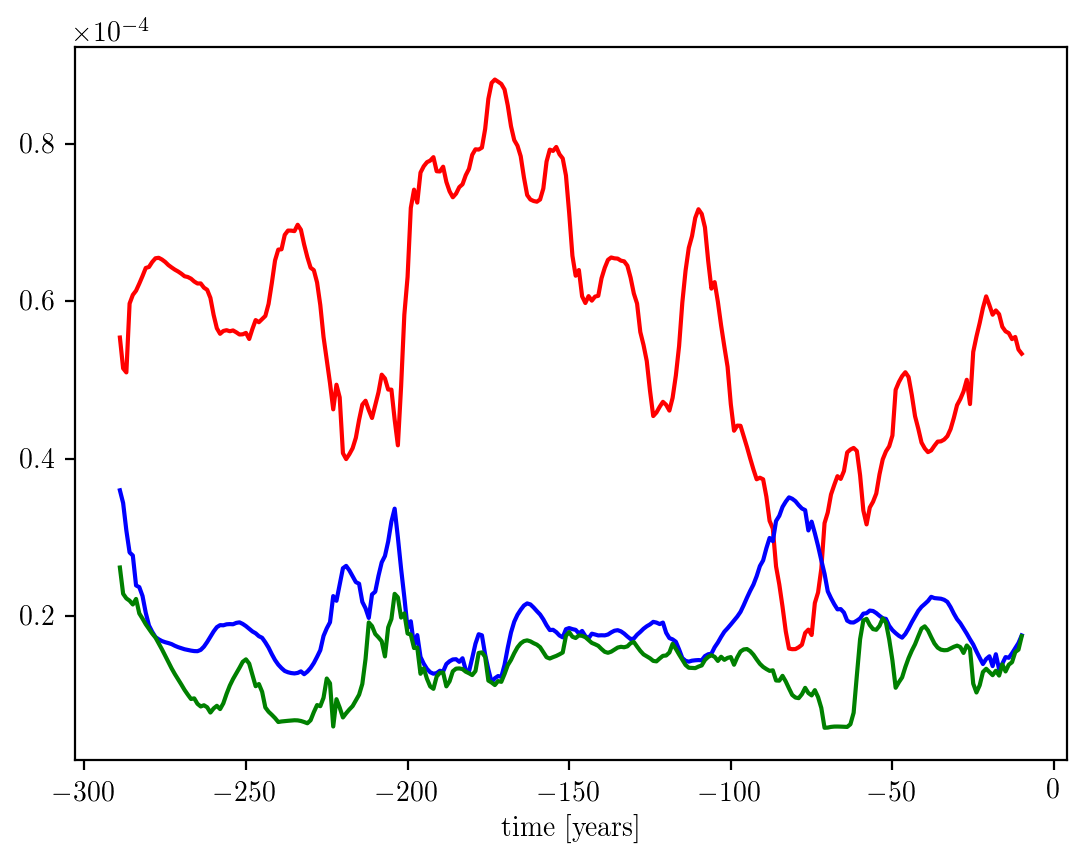
\includegraphics[width=1.0\textwidth]{figures/Amp_g3_2944}%
			\caption{The evolution of the amplitude of 3 strongest modes.}
			\label{fig:inv_exampleb}
		\end{subfigure}
		\caption{inversion of modes of a solution.}
		\label{fig:inv_example}
	\end{figure}
	To illustrate the inversion of modes, a particular solution is shown in figure (\ref{fig:inv_example}). The strongest mode of $g_3$ (violet dot) falls from the main curve to the curve below at around -87 Myr and then jumps back shortly after (Fig. \ref{fig:inv_examplea}). This short transition is evident from the evolution of their amplitudes (Fig. \ref{fig:inv_exampleb}). Amplitude of the main curve decreases during the first 90 Myr until it is smaller than the amplitude of the second mode, it then rises again and stays dominant for the rest of the integration time.
	
	The solution La2004 is also shown here to compare. The inversion of modes in the $g_4 - g_3 $ frequency is also visible at around $-87$ Myr in the spectrum of Earth's eccentricity (Fig. \ref{fig:2004a}). Nevertheless, the cause of inversion come from $g_4$ not $g_3$, $g_4$ occasionally jumps to a higher mode (numbering around 18.3 $''$/yr) for a short period of time and then jumps back (Fig. \ref{fig:2004b}).
	
	\begin{figure}[t]
		\centering
		\begin{subfigure}[t]{0.55\textwidth}
			%            \centering
			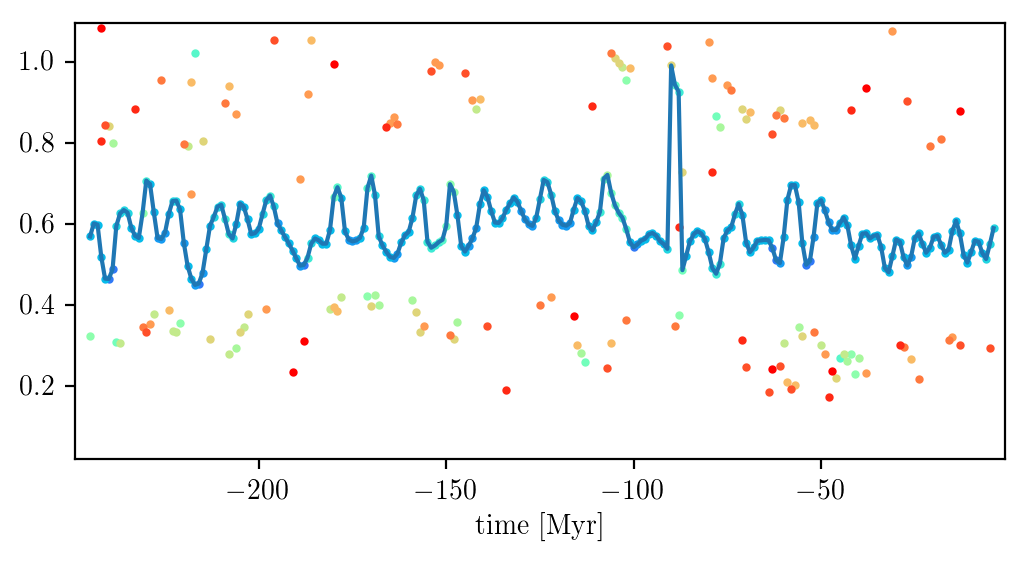
\includegraphics[width=1.0\textwidth,height=0.20\textheight]{figures/e_2004}%
			\caption{}
			\label{fig:2004a}
		\end{subfigure}%
		\begin{subfigure}[t]{0.55\textwidth}
			\centering
			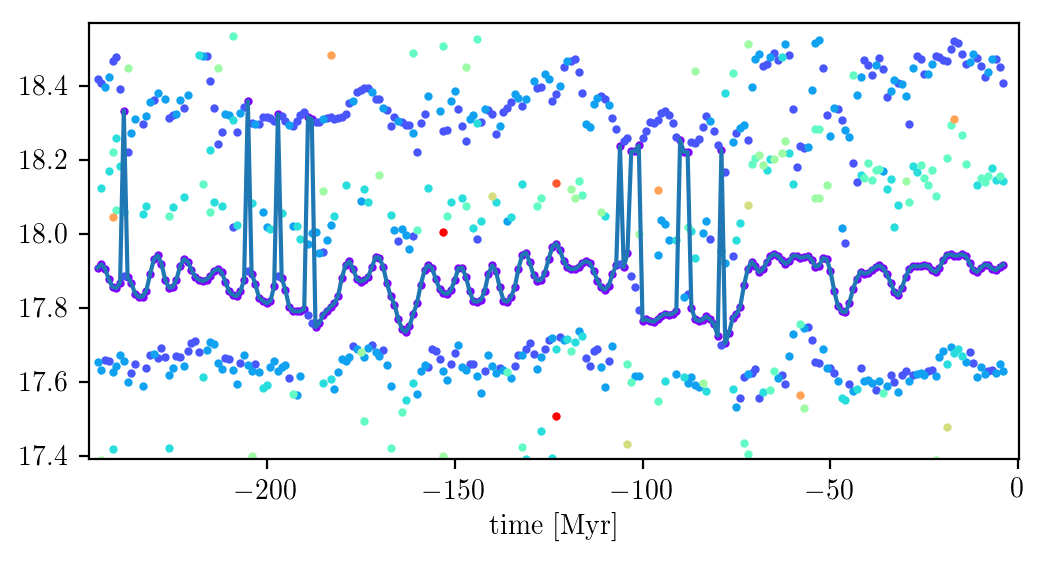
\includegraphics[width=1.0\textwidth,height=0.20\textheight]{figures/g4_2004}%
			\caption{}
			\label{fig:2004b}
		\end{subfigure}
		\caption{The evolution of the modes $g_4 - g_3$ (a) and $g_4$ (b). Violet indicates a strong mode while red indicates a weak mode, the shade of color in the middle indicate their strength accordingly. The curves go through the strongest mode at each time. The frequency analysis was done using the interval of 8 Myr. }
		\label{fig:2004}
	\end{figure}
	\subsection{Discussion}
	The dynamical origin of this inversion of modes is an open question. However, it is undoubtedly connected to the structure of resonances in the Solar System, especially between the Mars-Earth resonances: $\theta_1$ and $\theta_2$. The secular Solar System is presently in resonance $\theta_1$ with the primary mode of $g_3$ and $g_4$; it is also in resonance $\theta_2$ with second mode of $g_3$ (or $g_4$), but $\theta_2$ is not visible because the second mode is weaker than the main mode most of the time. Therefore, the back-and-forth jump between the main mode and the second mode of $g_3$ (or $g_4$) is actually the apparent transition between the resonance $\theta_1$ and $\theta_2$, which has been reported by many studies (\cite{laskar1990}, \cite{laskar2004} for example).
	
	\section{Conclusion}
	We have found several solutions that match better with the NH data, and a robust mechanism of the transition in Libsack record. From 10,000 numerical integrations of secular equation of 4 inner planets (Mercury, Venus, Earth, and Mars) over 300 Myr under the forcing of outer planets, we have also done a statistical analysis of fundamental frequencies and produced their PDF; we found a quantitative difference in the evolution of the PDF between the past and the future. The PDF of the frequencies differences between eccentricities of the numerical solutions and NH data PDF also presented. It is much more difficult to find a solution that matches the geological data from averaged equations than non-averaged ones. We speculate the cause of this disparity lies on the difference between the means of the secular PDF and the complete PDF. To test this, it is necessary to do a statistical comparison between the two. Yet, because it takes 4 months to obtain a single complete solution, several approximations have to be made to obtain a slightly-less complete but more efficient solution; moreover, more realistic secular equations could be used alternatively (the secular system at order 2 in planetary masses \citep{laskar1985} for example). With the purpose of assessing our current statistics, this will be the next step.
	
	\newpage
	\appendix
	\appendixpage
	\section{Laplace - Lagrange Hamiltonian} \label{App:H_LL}
	The matrices $ \mathbf{A} $ and $ \mathbf{B} $ in the Laplace-Lagrange Hamiltonian (\ref{H_sec}) are (N x N) real matrices. The components of $\mathbf{A}$ are \citep{laskar1995}:
	\begin{equation}
	\begin{aligned}
	\text{A}_{jj} &= \sum_{k=1}^{j-1} n_j \frac{m_k}{m_0} C_3 \left( \frac{a_k}{a_j} \right) + \sum_{k=j+1}^{N} n_j \frac{m_k a_j}{m_0 a_k} C_3 \left( \frac{a_j}{a_k} \right), \\ 
	\text{A}_{jk} &=\begin{cases}
	2n_j \frac{m_k}{m_0} \frac{a_j}{a_k} C_2  \left(  \frac{a_j}{a_k} \right) , & \text{if } j < k.\\ 
	2n_j \frac{m_k}{m_0} C_2 \left(  \frac{a_k}{a_j} \right)  , & \text{if } j>k.
	\end{cases}
	\end{aligned}
	\end{equation}
	The components of $\mathbf{B}$:
	\begin{equation}
	\begin{aligned}
	\text{B}_{jj} &= - \sum_{k=1}^{j-1} n_j \frac{m_k}{m_0} C_3 \left( \frac{a_k}{a_j} \right) - \sum_{k=j+1}^{N} n_j \frac{m_k a_j}{m_0 a_k} C_3 \left( \frac{a_j}{a_k} \right), \\ 
	\text{B}_{jk} &=  \sum_{k=1}^{j-1} n_j \frac{m_k}{m_0} C_3 \left( \frac{a_k}{a_j} \right) + \sum_{k=j+1}^{N} n_j \frac{m_k a_j}{m_0 a_k} C_3 \left( \frac{a_j}{a_k} \right). \\ 
	\end{aligned}
	\end{equation}
	The functions $C_2(\alpha)$ and $C_3(\alpha)$ are:
	\begin{equation}
	\begin{aligned}
	C_2 (\alpha) &= \frac{3}{8} \alpha b_{3/2}^{(0)} - \left( \frac{1}{4} + \frac{1}{4} \alpha^2 \right) b^{(1)}_{3/2}(\alpha), \\
	C_3 (\alpha) &= \frac{1}{4} \alpha b_{3/2}^{(1)},
	\end{aligned}
	\end{equation}
	where $b_k^{(j)}$'s are Laplace coefficients, which arises from the expansion of the inverse of a term related to distance; that is:
	\begin{equation}
	(1 + \alpha^2 - 2\alpha \cos \theta )^{-k} = \frac{1}{2} \sum_{j= - \infty}^{\infty}b_k^{(j)}(\alpha) \cos (j \theta),
	\end{equation}    
	Where $\alpha = a/a' <1$. Therefore,
	\begin{equation}
	b^{(j)}_k (\alpha) = \frac{2}{\pi} \int_{0}^{\pi} \frac{\cos(j\theta)}{(1 + \alpha^2 - 2\alpha \cos \theta )^k} d\theta.
	\end{equation}
	Higher order planetary Hamiltonian should be referred to \citep{laskar1995}
	
	\newpage
	\bibliographystyle{apalike}
	\bibliography{reference}
	
\end{document}

